%% august 16, 2021 edited by billf to be more like the current class lecture.
% image


\chapter{Statistical Image Models}
\label{chapter:stat_image_models}

%\reviewcomment{Readable but unfinished. Figures need to be reformatted and missing references.}

\section{Introduction}

Building statistical models for images is an active area of research in which there has been remarkable progress. Understanding the world of images and finding rules that describe the pixel arrangements that are likely to be present in an image and which arrangements are not seems like a very challenging task. What we will see in this chapter is that some of the linear filters that we have seen in the previous chapters have remarkable properties when applied to images that allow us to put constraints on a model that aims to capture what real images look like. 

First, we need to understand what we mean by a {\bf natural image}. An image is a very high dimensional array of pixels $\img \left[n,m\right]$ and therefore, the space of all possible images is very large. Even if you consider very small thumbnails of just $32\times32$ pixels and three color channels, with 8 bits per channel, there are more than $10^{7,398}$ possible images. Of course, most of them will just be random noise. \Fig{\ref{fig:spaces_real_images}} shows one image, with size $32\times32$ color pixels, sampled from the set of natural images, and on typical example from the set of all images. A typical sample from the set of all images is $32\times32$ pixels independently sampled from a uniform distribution. 

\begin{figure}
\centerline{
\includegraphics[width=.8\linewidth]{figures/statistical_image_models/spaces_real_images.eps}
} 
\caption{The space of natural images is just very small part of the space of all possible images. In the case of color images with $32\times32$ pixels, most of the space is filled with images that look like noise.} 
\label{fig:spaces_real_images}
\end{figure}


As natural images are quite complex, researchers have used simple visual worlds that retain some of the important properties of natural images while allowing the development of analytic tools to characterize them. 
In the last decade, researchers have developed large neural networks that learned generative models of images
and we discuss these models more in depth in \chap{\ref{chapter:generative_models}}. In this chapter we will focus on simpler image models as they will serve as motivation for some of the concepts that will be used later when describing generative models. 


\Fig{\ref{fig:worlds}} shows images that belong to different visual worlds. Each world has different visual characteristics. We can clearly differentiate images as belonging to any of these eight worlds, even if those visual worlds look like nothing we normally see when walking around. Explaining what makes images in the set of real images (\fig{\ref{fig:worlds}}[h]) different to images in the other sets is not a simple task. 

\begin{figure}
\centerline{
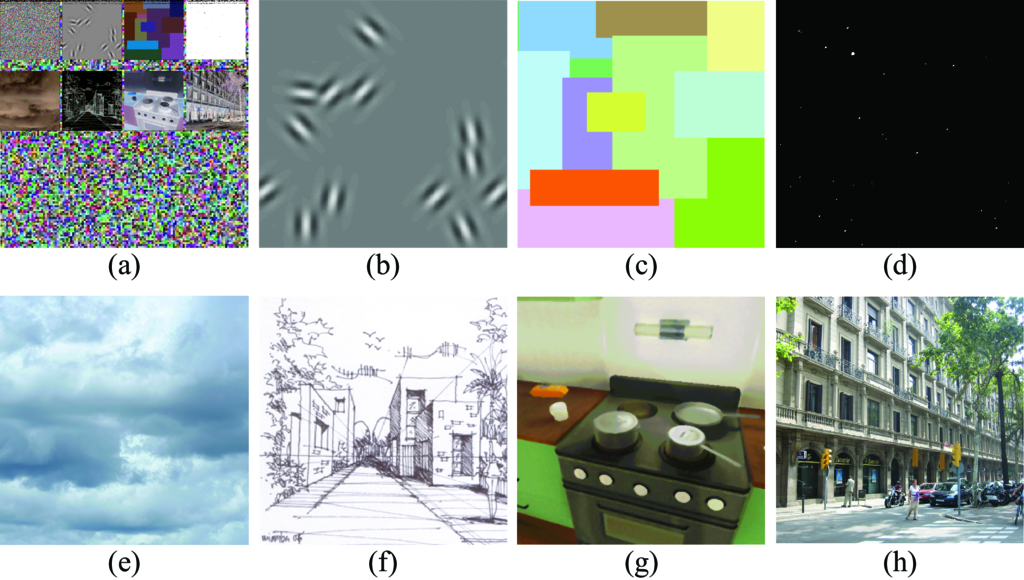
\includegraphics[width=1\linewidth]{figures/statistical_image_models/worlds.eps}
} 
\caption{Different visual worlds, some real, some synthetic. (a) White noise. (b) Gabor patches. (c) Mondrian. (d) Stars. (e) Clouds. (f) Line drawing. (g) Computer graphic imagery (CGI). (h) A real street.  All these worlds have different visual properties. There is even something that makes CGI images distinct from pictures of true scenes.} 
\label{fig:worlds}
\end{figure}



%
%The first world (fig.~\ref{fig:worlds}.a) is the world of white noise. It is the world that you get to see when you watch an old TV. Images in this world can be easily described by specifying the algorithm used to generate them: create and array of $n \times m$ color pixels and assign to each color component of each pixel a random number drawn from a uniform distribution between 0 and 255. In this world, all the images that belong to this world are very different in terms of the exact RGB values that make every pixel. But all the images look the same to the human visual system. 
%
%The second world (fig.~\ref{fig:worlds}.b) is the world of random Gabor patches. It is a visual world that one gets to see when reading papers on visual psychophysics. Again, an algorithm provides the perfect description for this world: select at random $N$ locations in the image and place at each location,a Gabor patch with a random orientation. These images look a lot more interesting to the human eye even though they contain a lot less detail than images from the first world.  
%
%The third world (fig.~\ref{fig:worlds}.c) is the world of Mondrian paintings. This world is more visually appealing. It contains structures that the eye loves. To the point that some people have made a lot of money by generating samples from this visual world. In its most simplistic form, the images that belong to this set can be described as a random set of squares with random sizes and locations. The squares are drawn in a random order, generating a random pattern of occlusions among them. 
%
%The fourth visual world (fig.~\ref{fig:worlds}.d) is the world of outer space images. This visual world, despite that it appears as being relatively simple, at least visually, it is not. However giving an exact algorithm to produce images from this set is quite challenging, but doable. One good approximation is to generate images by randomly placing a small number of small dots on a black background. A better algorithm will requite modeling star dynamics, gravity, etc.   
%
%The fifth visual world (fig.~\ref{fig:worlds}.e) is the world of clouds. This visual world is visually simple, but it is hard to put into words a description of how images of this set should be generated.  One can describe the images as "pictures of clouds" but that description will be hardly useful. 
%
%The sixth world (fig.~\ref{fig:worlds}.f) is the world of line drawings of real scenes. The images in this set contain a sparse set of thin dark lines on a white background. Going beyond that description is hard. One could also add that the lines are organized to depict real world places and that they seem to correspond to important boundaries of objects in the world. But that definition is not a good procedural description, and it also feels incomplete (some of the lines do not necessarily correspond to object boundaries).  
%
%The seventh world (fig.~\ref{fig:worlds}.g) is the world of realistic scenes rendered with cheap computer graphics. Because the images are generated with computer graphics, there is a procedure that one can follow to generate them. But the procedure lacks the simplicity of the previous visual worlds. The images in this set contain the complexity of real pictures. But there is something missing, something that makes that image to look like what it really is: a cheap CGI. 
%
%The eight world (fig.~\ref{fig:worlds}.h) is the set of typical images that one can take by taking pictures of the real world.  Explaining what makes images in this set different to all other images is not an easy task. 
%
%One important observation is that we can clearly differentiate images as belonging to any of these 8 worlds, even if those visual worlds look like nothing we normally see when walking around. 
%
In this chapter we will talk, in some way or another, about all these visual worlds. The goal is to present a set of models that can be used to describe images with different properties. We will describe models that can be used to capture what makes each visual world unique. 
% Even if the models we will discuss will not be as accurate as the models for the visual worlds a-c, we will show that the models can be descriptive enough to be useful in a number of applications.  
These models can be used to separate images into different causes, to remove noise from images, to predict the missing high-frequencies in blurry images, to fill in regions of missing image information due to occlusions, etc.




\begin{figure}[t]
\centerline{
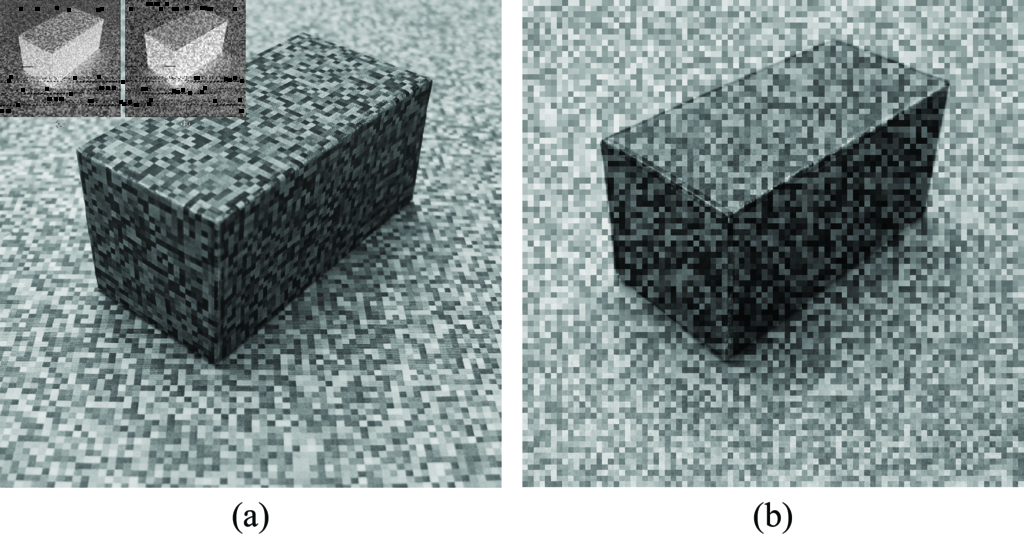
\includegraphics[width=1\linewidth]{figures/statistical_image_models/noiseInTheWorld.eps}
} 
\caption{Telling noise from surface texture. Which one is which?} 
\label{fig:noiseInTheWorld}
\end{figure}




%\section{Introduction}

% DOCUMENTS:
% lecture 3 (a bit)
% 
%Some history first: models used for TV? JPEG?

%\section{Retinex}
%
%How do you tell gray from white? This might seem like a simple question, but one remarkable aspect of vision is that even the perception of the simplest image and the measurement of the simplest quantity might be far from trivial. 
%
%\begin{figure}[htpb]
%\centerline{
%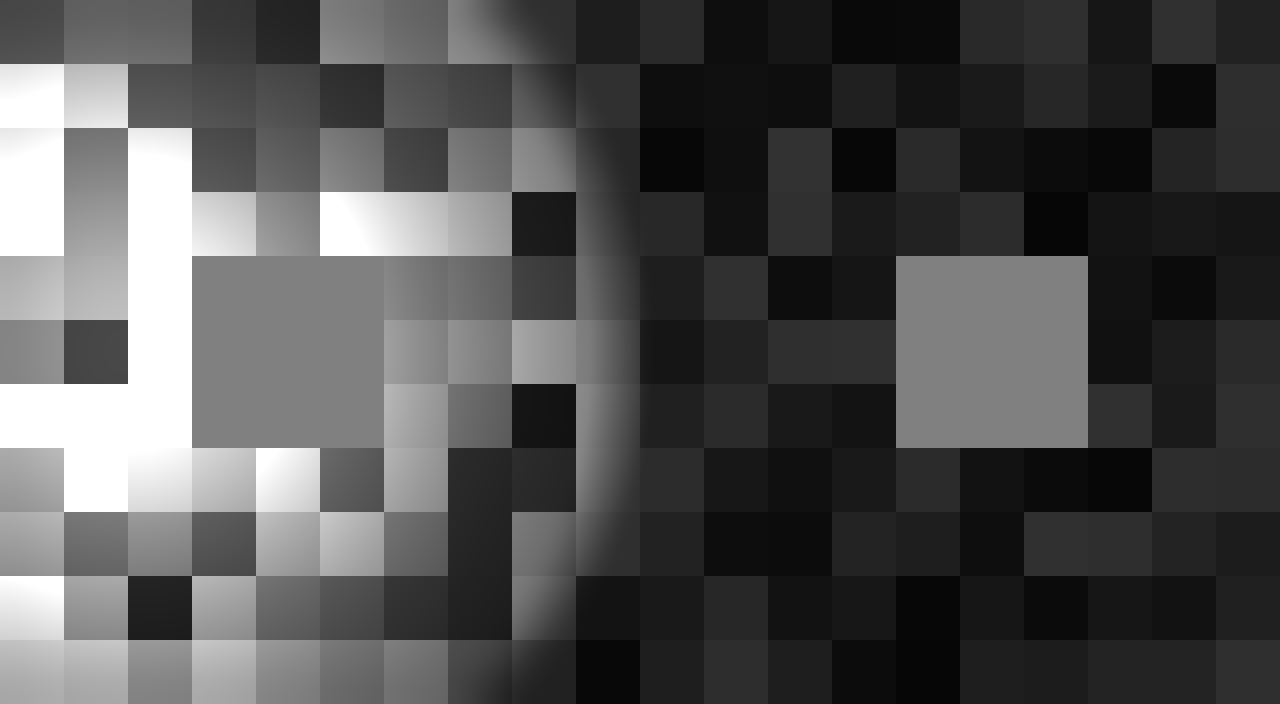
\includegraphics[width=1\linewidth]{figures/statistical_image_models/retinex.jpg}
%} 
%\caption{What happens if we see two patches of unknown reflectance, and each illuminated with two different light sources of unknown identity? Simultaneous contrast illusion.} 
%\label{fig:simultaneous}
%\end{figure}
%
%To understand that answering that question is not trivial, let's consider the structure of light that reaches the eye which is the input upon which our visual system will try to differentiate black from white. The amount of light that reaches the eye from painted piece of paper is the result of two quantities: the amount of light reaching the piece of paper, and the reflectance of the surface (what fraction of the light is reflected back into space and what fraction is absorbed by the material).
%
%
%%The brightness of a patch is a function of the light reaching a surface and how much light is reflected by that surface. Under the same illumination, one patch might appear darker than another if it reflects less light. On the other hand, if one patch received more light than other identical patch, the first patch will appear brighter. Therefore, 
%
%
%
%If two patches receive the same amount of light, then we will perceive as being darker the patch that reflects less light. But what happens if we change the amount of light that reaches the scene? What if we increase the amount of light projected on top of the dark patch, what will be see now? What will happen if we have two patches on the same scene each of them receiving different amounts of light? How does the visual system decide what white is and how does it deal with changes in the amount of light illuminating the scene? The visual system is constantly trying to estimate what the incident illumination is and what are the actual reflectances of the surfaces present in the scene. 
%
%If our goal is to estimate the shade of gray of a piece of painted paper, then the quantity that we care about is the reflectance of the surface. But, what happens if we see two patches of unknown reflectance, and each illuminated with two different light sources of unknown identity?  How does the visual system manages to infer what the illumination and reflectances are?
%
%Visual illusions are a way of getting to feel how our own visual system processes images. To experience how this estimation process works let's start considering a very simple image as shown in fig.~\ref{fig:simultaneous}. This image shows a very simple scene formed by a surface with a set of squares of different gray levels illuminated by a light spot oriented towards the left. Our visual system, tries to estimate the two quantities: the reflectance of each square and the illumination intensity reaching each pixel.  
%
%Let's think of the image formation process. The surface is made of patches of different reflectances $R(x,y) \in (0,1)$. Each location receives an illumination $L(x,y)$. The observed brightness is the product:
%\begin{equation}
%\img(x,y) = R(x,y) \times L(x,y) 
%\end{equation}
%
%Despite that what reaches the eye is the signal $\img(x,y)$, our perception is not the value of $\img(x,y)$. In fact, the squares 1 and 2 in fig.~\ref{fig:simultaneous} have the exact same values of intensity but we see them differently which is generally explained by saying that we discount (at least partially) the effects of $L(x,y)$. 
%
%But how can we estimate $R(x,y)$ and $L(x,y)$ by only observing $\img(x,y)$? One of the first solutions to this problem was the Retinex algorithm proposed by Land and McCann. Land and McCann observed that it is possible to extract $R$ and $L$ from $\img$ if one takes into account some constraints about the expected nature of the images $R$ and $L$. Land and McCann noted that if one considers two adjacent pixels inside one of the patches of uniform reflectance, the difference between the two pixel values will be very small as the illumination, even if it is nonuniform, will only produce a small change in the brightness of the two pixels. However, if the two adjacent pixels are in the boundary between two patches of different reflectances, then the intensities of these two pixels will be very different. 
% 
%The Retinex algorithm works by first extracting x and y spatial derivatives of the image $\img(x,y)$ and then thresholding the gradients.  First, we transform the product into a sum using the $\log$:
%
%\begin{equation}
%\log \img(x,y) = \log R(x,y) + \log L(x,y) 
%\end{equation}
%Taking derivatives a long $x$ and $y$ is now simple:
%\begin{equation}
%\frac{\partial \log \img(x,y)}{ \partial_x} = \frac{\partial \log R(x,y)}{ \partial_x} + \frac{\partial \log L(x,y)}{ \partial_x} 
%\end{equation}
%
%Any derivative larger that the threshold is assigned to the reflectance image $R(x,y)$ and the ones smaller than a threshold are assigned to the illumination image $L(x,y)$
%
%\begin{equation}
%\frac{\partial \log R(x,y)}{ \partial_x} =  \left\{
%\begin{array}{rl}
%\frac{\partial \log \img(x,y)}{ \partial_x} & \text{if} ~  \left| \frac{\partial \log \img(x,y)}{ \partial_x} \right|>T\\
%0 ~~~~~~~~& \text{otherwise}
%\end{array} \right.
%\end{equation}
%
%\begin{figure}[htpb]
%\centerline{
%\includegraphics[width=1\linewidth]{figures/statistical_image_models/retinex_solution_b.eps}
%} 
%\caption{Derivatives classified into reflectance or luminance components.} 
%\label{fig:simultaneous2}
%\end{figure}
%
%and doing the same thing from $ \partial_y$. Then, the image $\log R(x,y)$ is obtained by integrating the gradients and exponentiating the result. Finally, the illumination can be obtained as $L(x,y) = \img(x,y)/R(x,y)$.
%
%\begin{figure}[htpb]
%\centerline{
%\includegraphics[width=1\linewidth]{figures/statistical_image_models/retinex_solution_a.eps}
%} 
%\caption{Recovered components.} 
%\label{fig:simultaneous3}
%\end{figure}
%
%Note that the illumination derivatives have much lower magnitude than the reflectance derivatives, however they extend over much larger spatial regions which makes that once they are integrates, changes in brightness due to no-uniform illumination might be larger than changes due to variations in reflectance values. 
%
%Despite the simplicity of this approach it works remarkable well with images like the ones shown in fig.~\ref{fig:simultaneous} and also with a number of real images. However, the algorithm is limited and it is easy to make it fail in situations were the visual system works as we will see later in more depth.
%
%The Retinex algorithm works by making assumptions about the structure of the images it tries to separate. The underlying assumption is that the illumination image $L(x,y)$ varies smoothly and the reflectance image $R(x,y)$ is composed of uniform regions separated by sharp boundaries. These assumptions are very restrictive and will limit the domain of applicability of such an approach. Understanding the structure of images in order to build models such as Retinex has been the focus of a large amount of research. This chapter will introduce some of the most important image models.
%
%The recovered brightness is stronger than what we perceive. There are a number of reasons that weaken the perceived brightness. The effect is bigger if the display occupies the entire visual field. Right now the picture appears in the context of the page which also affects the estimation of the illumination. Also, the two larger squares do not seem to group well with the rest of the display, as if they were floating in a different plane. And finally, for such a simple display, the visual system does not fully separate the perception of both components. 
%

%CNNs try to learn what to do with images to solve a task.

%In this chapter, we describe techniques in which researchers try to derive how to do process images using simple principles about the real world. Under some assumptions the solutions are optimal (although the assumptions are often wrong).




%Example 1: Retinex: Mondrian world with a illumination ramp. 


%FROM TED: Land and McCann began by considering the nature of
%scenes and images. They argued that reflectance tends to be
%constant across space except for abrupt changes at the transitions
%between objects or pigments. Thus a reflectance
%change shows itself as step edge in an image, while illuminance
%will change only gradually over space. By this argument
%one can separate reflectance change from illuminance
%change by taking spatial derivatives: high derivatives are due
%to reflectance and low ones are due to illuminance.
%The Retinex model applies a derivative operator to the
%image, and thresholds the output to remove illuminance variation.
%The algorithm then reintegrates edge information over
%space to reconstruct the reflectance image.
%
%Helmholtz, who argued that perception is the product of
%unconscious inference. His dictum was this: what we perceive
%is our visual systemÕs best guess as to what is in the
%world. The guess is based on the raw image data plus our
%prior experience. In the Helmholtz view, lightness constancy
%is achieved by inferring, and discounting, the illuminant.
%
%We use the term atmosphere to
%refer to the combined effects of a multiplicative process
%(e.g., illuminance) and an additive process (e.g., haze). It turns out that most physical effects will
%lead to linear transforms. Therefore the combined effects can
%be captured by a single linear transform (characterized by
%two parameters). This is what we call an atmosphere.

% Retinex works by thresholding the gradients and assigning
%the gradients below the threshold to the gradients of the
%illumination image.



%Example 2:

%This problem has an even simpler version. 

% Gray scale constancy



% There is an analogy to make with language models. They also look for generative models of language. The statistical models are very similar. 

%TO ADD:
%
%- Intrinsic images
%
%- Frameworks of illumination
%
%- Anchor theory
%
%- Failures of the simple mechanism: Kersten images
%
%- What seems white now, might appear gray if something whiter appears on the same scene. 


\section{How Do We Tell Noise from Texture?}

How do we tell noise from texture? \Fig{\ref{fig:noiseInTheWorld}} shows two scenes:  one image is corrupted with additive stationary noise added on top of the image, the other image contains one object textured with a pattern that looks like noise. Can you tell which one is which? Where is the noise? Is it in the image or in the world?  


Stationary image noise\footnote{Additive stationary noise is noise with statistical properties independent of location that is added to an observation. Check \sect{\ref{sec:image_denoising_gaussian_model}} for a more precise definition.} is independent of the content of the scene, it is not affected by the object boundaries, it does not deform following the three-dimensional (3D) orientation of the surfaces, and it does not change frequency with distance between the camera and the scene. If the noise was really in the world, stationary noise would require a special noise distribution that conspires with the observer viewpoint to appear stationary. 

Noise is an independent process from the image content, and our visual system does not perceive noise as a strange form of paint. One important task is image processing it image denoising. Image denoising consists in removing the noise from an image automatically. This is equivalent to being able to separate the image into two components, one looking like a clean uncorrupted picture and the second image containing only noise. Statistical image models try to do this and more. 

\marginnote{The original images from
\fig{\ref{fig:noiseInTheWorld}}.\\[6pt]
\centerline{
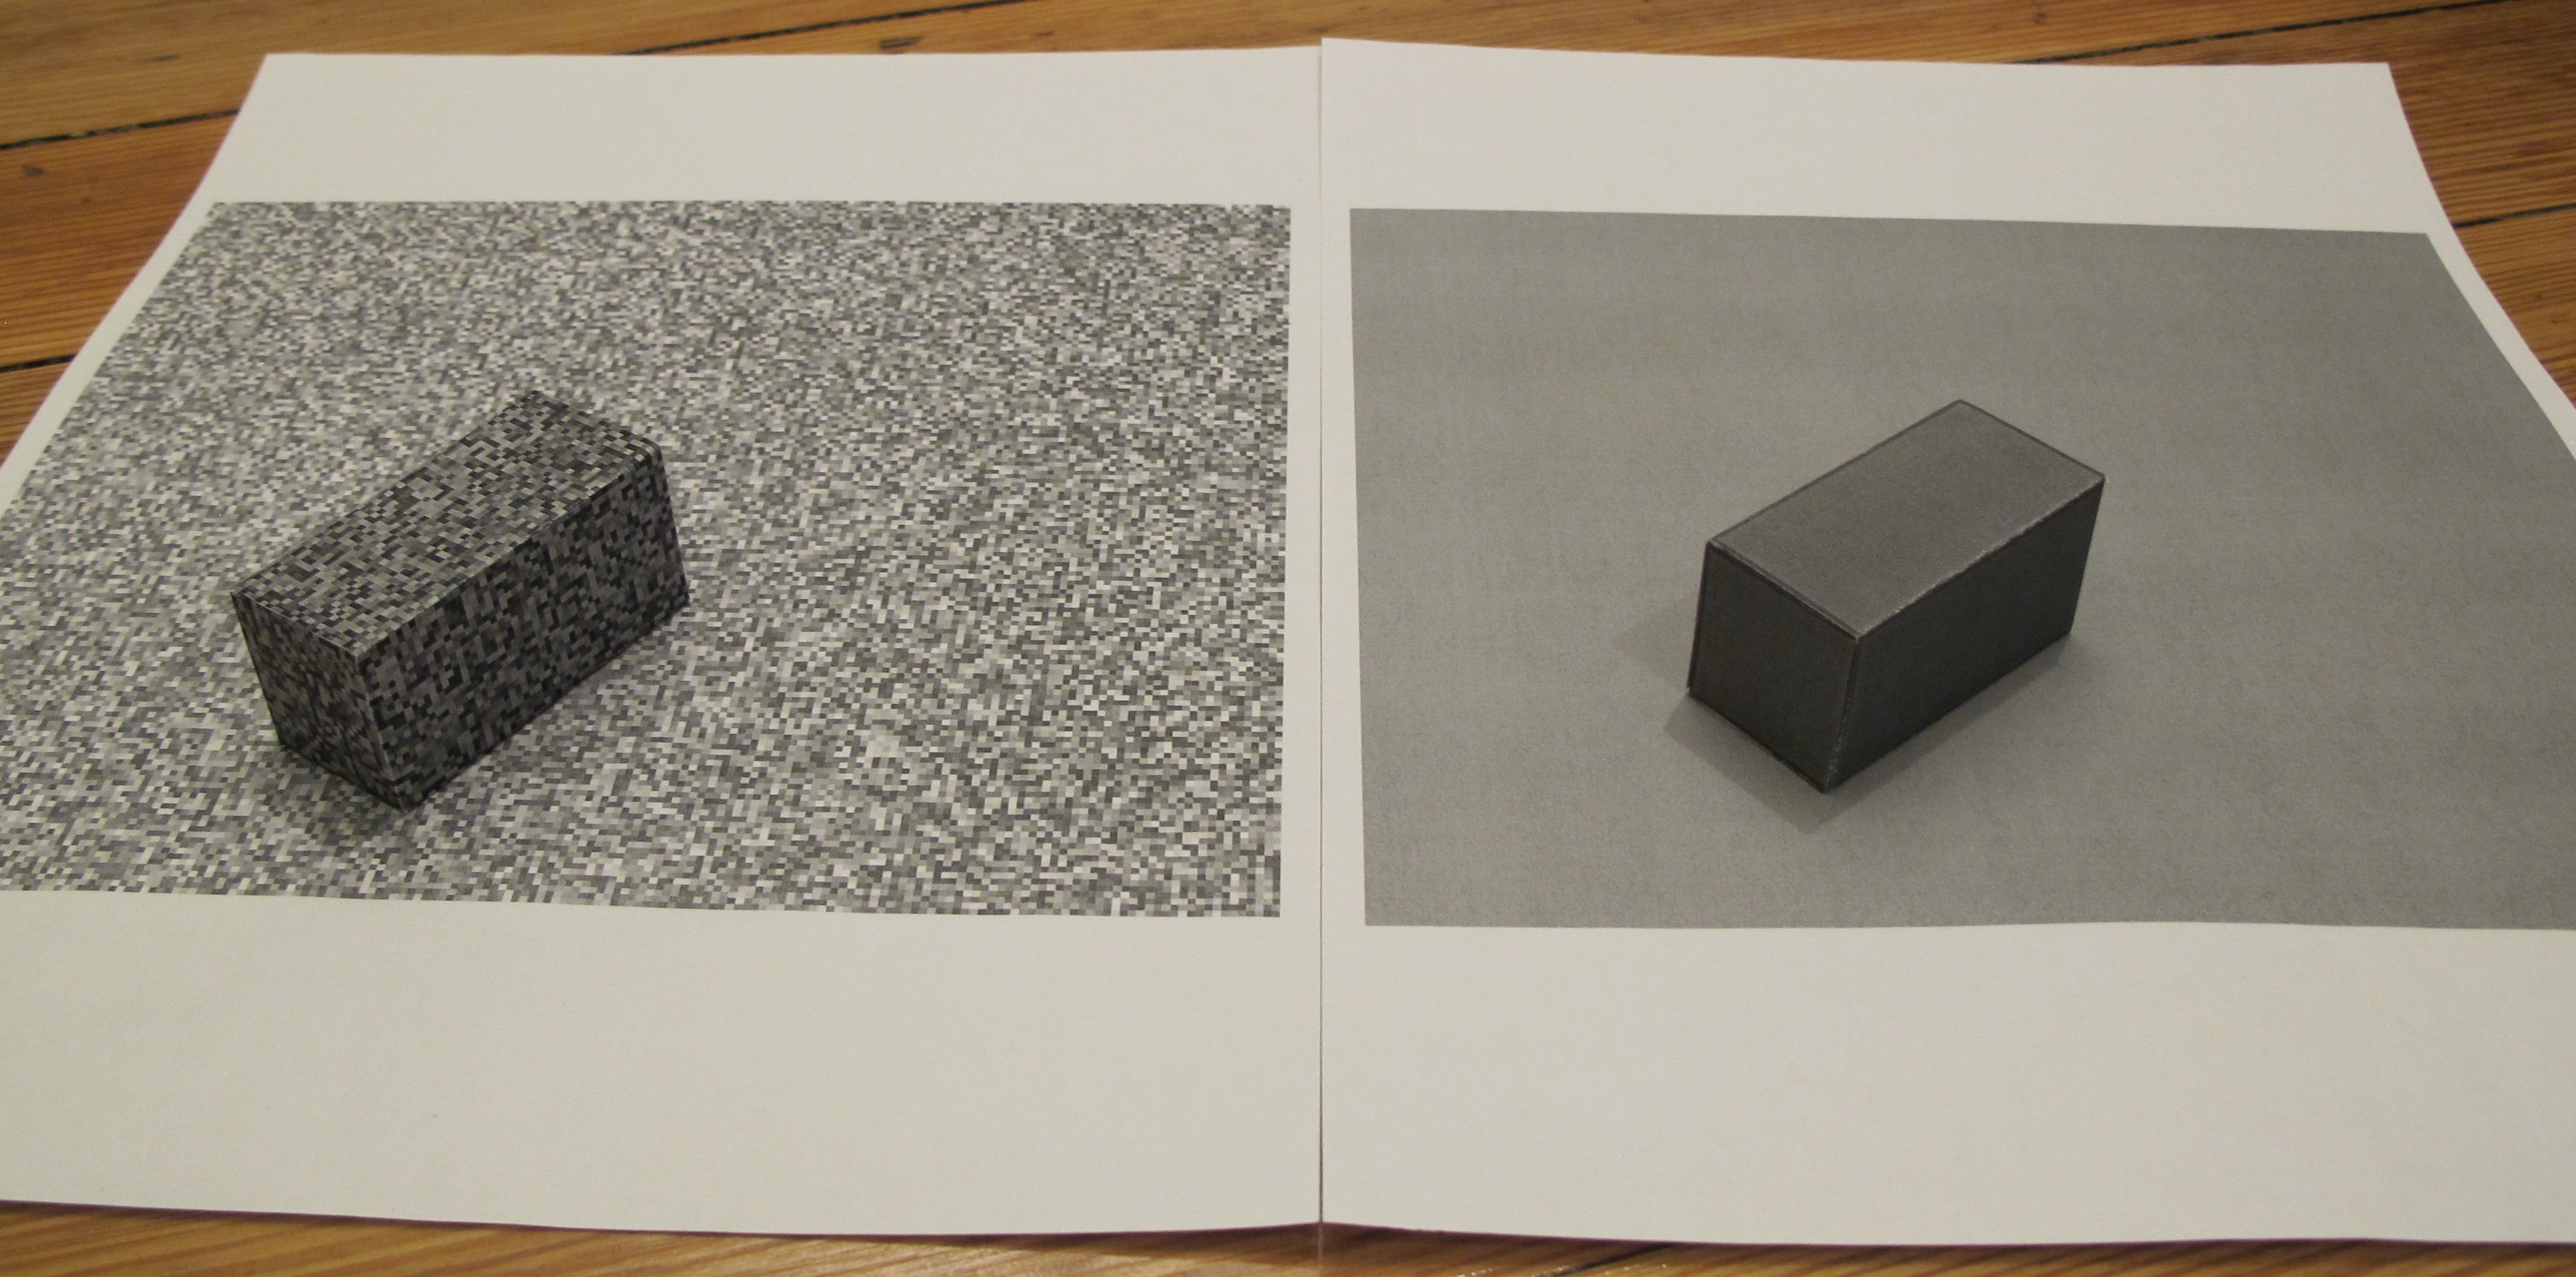
\includegraphics[width=.8\linewidth]{figures/statistical_image_models/cubes_with_and_without_noise.jpg}
}
\\[6pt]
\Fig{\ref{fig:noiseInTheWorld}}{b} has noise added. 
}[-.3in]

%
%\begin{figure}[htpb]
%\centerline{
%\includegraphics[width=1\linewidth]{figures/statistical_image_models/mixtures3_a.eps}
%} 
%\caption{The goal is to separate each image into several images.} 
%\label{fig:mixtures}
%\end{figure}
%
%One of the reasons why it is interesting to understand the properties of different sets of images is because many perceptual tasks can be formulated as separating an input image into a collection of images, each one describing a different image property. %Figure \ref{fig:mixtures} shows three additional examples of images that have are made of multiple components.  
%
%%The first example shows a normal photograph corrupted by noise. 
%
%\begin{figure}[htpb]
%\centerline{
%\includegraphics[width=1\linewidth]{figures/statistical_image_models/mixtures3_noise.eps}
%} 
%\caption{The goal is to separate each image into several images.} 
%\label{fig:mixtures}
%\end{figure}
%
%\begin{equation}
%\img_n(x,y) = \img(x,y) + n(x,y)
%\end{equation}
%
%Our visual system is able to notice that this image is not normal and that it is corrupted by noise. We do not perceive this scene as being composed by objects covered with a strange form of paint. We see that there is {\em noise} and it is not supposed to be there, it is not part of the real scene. What we will like is to be able to remove the noise from the image automatically. This is equivalent to be able to separate the image into two components, one looking like a clean uncorrupted picture of a street and the second image containing only noise. 
%

%
%The second example shows a blurry image. 
%
%\begin{figure}[htpb]
%\centerline{
%\includegraphics[width=1\linewidth]{figures/statistical_image_models/mixtures3_blur.eps}
%} 
%\caption{The goal is to separate each image into several images.} 
%\label{fig:mixtures}
%\end{figure}
%
%\begin{equation}
%\img_b(x,y) = \img(x,y) \circ g(x,y) 
%\end{equation}
%
%This image can be decomposed into a full resolution image from which we remove the high spatial frequencies from it. Again, we do not perceive the blurry image as a normal picture of a scene composed by objects with fuzzy boundaries. 
%
%
%and the third image is the sum of two normal images (additive transparency). Again, we have a very vivid impression of transparency. 
%
%\begin{figure}[htpb]
%\centerline{
%\includegraphics[width=1\linewidth]{figures/statistical_image_models/mixtures3_transparency.eps}
%} 
%\caption{The goal is to separate each image into several images.} 
%\label{fig:mixtures}
%\end{figure}
%
%\begin{equation}
%\img_t(x,y) = \img_1(x,y) + \img_2(x,y) 
%\end{equation}
%
%Separating an image into different causes it is an important vision task.  It is important to note that the separation into these components does not rely on our ability to recognize objects and scenes (at least not totally). It seems to rely on more basic mechanisms. These tasks can not be solved without making some assumptions about the nature of the composing images. 

%The problem we are trying to solve is like trying to find $a$ and $b$ given the next equation:
%\begin{equation}
%1 = a \times b
%\end{equation}
%
%Compare this with the prototypical graphics problem: here are two numbers $a$ and $b$;  what is their product?
%
%In the rest of the chapter we will see models of images that will provide useful tools to separate images into components. 
%
%
%
%
%\section{Bayesian inference}
%
%In many situations in vision we observe some complicated function of the world 
%\begin{equation}
%observation = f(world)
%\end{equation} 
%It would be nice if one could simply do $world = f^{-1}(observation)$, and, in some cases, this is possible. But in general, inverting this function might be very difficult, or ill-posed. As we saw before, in many important cases, there are multiple $worlds$ that give raise to the same $observations$. We need to find a way of inverting this function. Bayesian inference provides the set of tools to regularize the solution and to add priors. It also provides the tools to deal with uncertainty due to noise in our observations. Let's see how we can use Bayesian inference to find the solution to the typical vision problem $ab=1$.
%
%%Introduce Bayes
%
%%Introduce notation with random variables
%
%%Talk about inference and Helmholtz
%
%%A way of dealing with uncertanty
%
%%A way of doing function inversion when the problem is under constrained. One example: the typical vision problem $ab=1$:
%
%%\example{Grayscale constancy}
%%
%%
%%Conclude making a simple image example to help introducing the interest of a model of an image prior. In the case of images, we can have:
%%
%%\begin{equation}
%%p(\img) = 
%%\end{equation}
%%
%%
%%The problem $ab=1$ is quite typical in vision. Let's consider a real vision problem. 
%%
%%Let's consider the image from figure XXX. This image is composed by a set of squares with different levels of gray. One of them is perceived as white. However, how is that we see that square as being white? Despite that this might seem trivial, it is not once we consider how the image that reaches our eye is formed.
%%
%%What we see is the product of
%%
%%\begin{equation}
%%[k_1, k_2, ..., k_n] = a [b_1,b_2, ..., b_N]
%%\end{equation}
%% To find $L$ and the sequence of reflectances $b_1, ..., b_N$ we are going to need to make some assumptions.
%% 
%%Suppose all reflectances $b_i$ are uniformly distributed between 0 and 1.  
%%
%%\begin{equation}
%%p(b_1, b_2, ..., b_N) =   \left\{
%%\begin{array}{rl}
%%1 & \text{if } 0<b_i <1\\
%%~ & ~\\
%%0 & \text{otherwise}
%%\end{array} \right.
%%\end{equation}
%%
%%
%%Suppose you observe N image intensities, which is the product of those N reflectance draws
%%times some unknown illumination $L$ (with $L>0$).  If we can estimate the reflectance
%%of the brightest patch, then we can calculate the unknown illumination
%%value, and then the reflectance of every patch.  
%%
%%
%%For N reflectance draws, we can calculate the probability that the
%%brightest of those N draws has a reflectance of x.  That's the same as
%%the probability that every reflectance draw is x or lower, which is
%%$x^N$.  As the number of observed reflectances, N, gets bigger and
%%bigger, it becomes a better and better bet that the brightest of those
%%patches is white. This is true even for an arbitrary distribution of reflectances between 0 and 1. 
%%
%%why not to look for the average gray? That could be more reliable than everything as it would not depend on any maximum value. I think that the problem of using the average is that then it will not be distribution independent. Using the max value is distribution independent.
%%
%%It's interesting to think through what breaks the symmetry (black/white):  why not look for the blackest patch and call it "black".     (a) there is no value of "black", as there is a value for white, 1.0.  Should it be a reflectance of 0.001?  0.00001?   and (b) so then knowing which intensity is black doesn't tell you what the light intensity is, because you can't divide the observed intensity by the unknown value of black to find the illumination intensity.
%%
%%
%%
%%Using the average gray is certainly a standard algorithm.  I believe the reference for that is Buchbaum,
%%G. Buchsbaum. A spatial processor model for object colour
%%perception. J. Franklin Inst., 310:1{26}, 1980.
%%
%%And I guess a reference for bright=white could be some Retinex paper.  They don't justify it, but they certainly use that assumption.
%%So maybe this:  E. H. Land. The retinex theory of color vision. Sci. Am.,
%%237(6):108{128}, 1977
%%
%%
%%And indeed, our visual system seems to follow that reasoning.  If you see a greater variation of patch values, intensity illusions that rely on the bright=white assumption get stronger and stronger (some of Ted's brightness illusions).
%%
%%FIGURE: Frameworks of illumination: figure with two sets of randomly colored patches, with a division between them. In the left [0,0.5] and in the right [0,1]. We will see a vertical shadow. And we will see the right white from each side. 
%%
%%
%%
%%\begin{figure}[htpb]
%%\centerline{
%%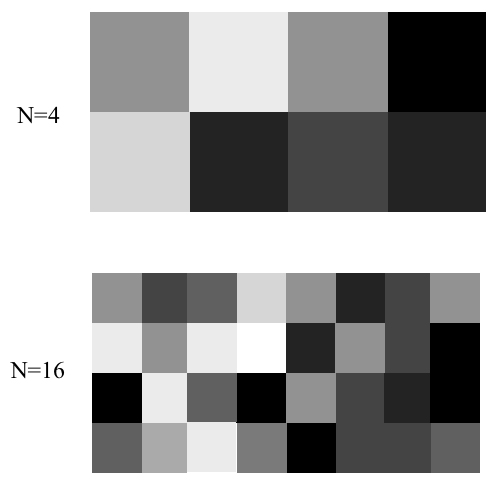
\includegraphics[width=.6\linewidth]{figures/statistical_image_models/chips.jpg}
%%} 
%%\caption{Here is an example showing the effect of the number of independent samples, N, on the estimate of illuminations and reflectances.  For N=4, there aren't quite enough samples to decide on regions of uniform illumination, while for N=16, you start to get the sense that the right hand side is in shade.  Maybe including N=64 would make it completely clear.} 
%%\label{fig:chips}
%%\end{figure}
%%
%%
%
%%\section{Gestalt}
%%
%%%The
%%%key concepts include grouping, belongingness, good continuation,
%%%proximity, and so on.
%%
%%Can we introduce grouping theories as particular instances of statistical image models?
%%
%%
%%The problem is that to use these statistics we need to detect some tokens on the image (edges, junctions, ...). We will see how to do this later, but even with the most accurate detectors, the output is still unreliable. In the rest of the chapter we will study a different class of statistical image models that do not require taking premature decisions about the image content. 
%
%%\section{Accidental alignments}
%%
%%
%%where do we talk about accidental alignments? Isn't this also part of statistical image models?
%%
%%This is a good example on the power of statistical models to solve hard tasks. 
%%
%
%




%% \section{A sequence of statistical models of images}

There is a significant interest in building image models that can represent whatever makes real photographs unique relative to, say, images that just contain noise. One way of building an image model is by having some procedural description, for instance a list of objects with locations, poses, and styles and a rendering engine, just as one would do when writing a program to generate CGI. One issue with this way of modeling images is that it will be hard to use it, and will require having an exhaustive list of all the things that we can find in the world. We will see later that the apparent explosion in complexity should not stop us. 

% % Drawing the blocks of first level:
% \centerline{
% \tikzset{
%   block/.style    = {draw, thin, rectangle, minimum height = 2.5em,  minimum  width = 2.5em},
%   sum/.style      = {draw, circle, minimum size=.4cm}, % Adder
%   input/.style    = {coordinate}, % Input
%   output/.style   = {coordinate}, % Output
%   x/.style   = {coordinate} % Output
% }
% \begin{tikzpicture}[auto, thin, node distance=1.2cm, >=triangle 45]
% \draw
% 	node [] (x0p) {$x$}
% 	node [block, right of=x0p] (f) {$f$}
% 	node [right of=f, node distance=2.6cm] (out) {$p(x \in World)$};
%       % Joining blocks. 
%	\draw[->](x0p) -- node {} (f);
%	\draw[->](f) -- node {} (out);
% \end{tikzpicture}
% }
However, there is another way of building image models. In the rest of this chapter we will study a very different approach that consists of building statistical models of images that try to capture the properties of small image neighborhoods. Statistical models are also foundational in other disciplines such as natural language modeling. 
Here we will review models of images of increasing complexity, starting with the simplest possible neighborhood: {\em the single pixel}.


\section{Independent Pixels}
\label{sec:independent_pixels}


%\subsection{Histograms}

The simplest image model will consist in assuming that all pixels are independent and their intensity value is drawn from some stationary distribution (i.e., the distribution of pixel intensities is independent of the location in the image). We can then write the probability, $p_{\theta}(\boldimg)$, of an image, $\img [n,m]$ with size $N \times M$, as follows:
\begin{equation}
p_{\theta}(\boldimg) = \prod_{n=1}^{N} \prod_{m=1}^{M} p_{\theta}\left(\img [n,m] \right)
\label{eq:histmodel}
\end{equation}
We use $p_{\theta}$ to denote a parameterized probability model. The vector $\theta$ contains the parameters and can be fitted to data using maximum likelihood or other loss functions. We will see many variants of this probability model here and in the following chapters. 

One way of assessing the accuracy a statistical image model is to sample from the model and view the images it produces. This will require knowing the distribution $p_{\theta}\left(\img [n,m] \right)$. 

What we can do is to take one image from one of the visual worlds that we described in the introduction, and then estimate the model $p_{\theta}\left(\img [n,m] \right)$, as illustrated in \fig{\ref{fig:model_training_vs_sampling}}. 

\begin{figure}
\centerline{
\includegraphics[width=.75\linewidth]{figures/statistical_image_models/model_training_vs_sampling.eps}
} 
\caption{Fitting a statistical image model to a set of training images. Once the model is learned we can use the model to sample new images.} 
\label{fig:model_training_vs_sampling}
\end{figure}



In the case of discrete gray-scale images with 256 gray levels, we can represent the distribution $p_{\theta}$ as vector of 256 values indicating the probability of each intensity value. In the case of considering color images with 256 levels on each channel (i.e., 8 bits per channel) we will have $256^3$ bins in the color histogram.
\index{Color histogram}

\marginnote{The {\bf histogram}, $h(c)$, of a gray scale image, $\img[n,m]$, contains the number of times each intensity value, $c$, appears in the image: 
\begin{equation*}
h(c) = \sum_{n,m} \mathbbm{1} \left( \img[n,m] = c \right)  
\end{equation*}
The length of $\mathbf{h}$ is equal to the number of distinct intensity values.}[-.95in]\index{Image histogram}

The parameters, $\theta$, of the distribution are those 256 (or $256^3$ for color) values.  
If we are given a set of images, we can estimate the vector $\theta$ as the average histogram of the images. 
We can also estimate the model from a single image. We can then sample new images based on \eqn{\ref{eq:histmodel}}. In order to sample a new image, we will sample each pixel independently using the intensity distribution given by the training set. 

The procedure for four training images is shown in \fig{\ref{fig:model_hist_example}}. As illustrated in \fig{\ref{fig:model_hist_example}}, the process starts by computing the average color histogram for the four images. Then, we sample a new image by sampling every pixel from the multinomial defined by the $p_{\theta}$. \marginnote{In the multinomial model, the probability that the image in location $(n,m)$ has the value $k$ is $p_{\theta}(\img [n,m] = k) = \theta_k$. In the case of color images, in this model, $k$ will be one of the $256^3$ possible color values.}[-1in]


\begin{figure}
\centerline{
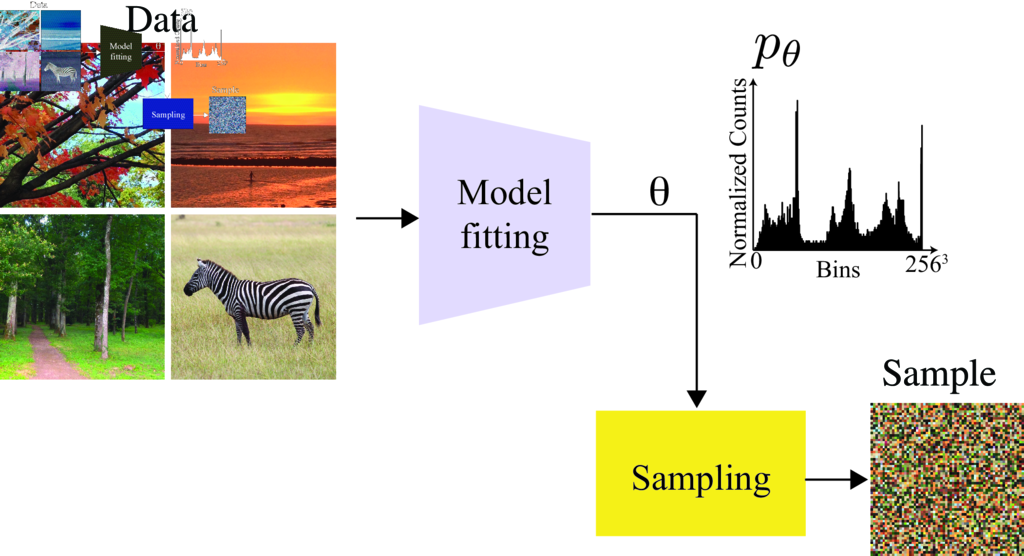
\includegraphics[width=1\linewidth]{figures/statistical_image_models/model_hist_example2.eps}
} 
\caption{Estimation of the image model parameters using one image, and then sampling a new image by sampling pixels independently using the histogram of the training image.}
\label{fig:model_hist_example}
\end{figure}

 \Fig{\ref{fig:histMatch}} shows four pairs of images with matched color histograms. We can see that this simplistic model is somewhat appropriate for pictures of stars (although star images can have a lot more structure), but it miserably fails in reproducing anything with any similarity (besides the overall color) to any of the other images. The failure of color histograms as a generative model of images should not be surprising as treating pixels as independent observations is clearly not how images work. 


\begin{figure}
\centerline{
\includegraphics[width=1\linewidth]{figures/statistical_image_models/4_examples_images.eps}
} 
\caption{Examples of images and corresponding random samples with the same distribution of pixel intensities. Only the image with stars (a) has some visual similarity with the randomly sampled image.}
\label{fig:histMatch}
\end{figure}

As a generative model of images, this model is very poor. However, this does not mean that image histograms are not important. Manipulating image histograms is a very useful operation.  Given two images $\boldimg_1$ and $\boldimg_2$ with histograms $\mathbf{h}_1$ and $\mathbf{h}_2$, we look for a pixelwise transformation $f\left(\img [n,m] \right)$ so that the histogram of the transformed image, $f\left(\img_1 [n,m] \right)$, matches the histogram of $\boldimg_2$. There are many ways in which histograms can be transformed. One natural choice is a transformation that preserves the ordering of pixels intensities. 

\Fig{\ref{fig:illumination}} shows examples of spheres that are reflecting some complex ambient illumination.  This is an example that illustrates the perceptual importance of simple histogram manipulations. The two spheres on the left are the two original images. The ones on the left are generated by modifying the image histograms to match the histogram of the opposite image.  The figure shows that by simply changing the image histogram we can transform how we perceive the material of each sphere: from shiny to matte \cite{Fleming2001}.
The sphere was first rendered with two illumination models: from a campus photograph (\fig{\ref{fig:illumination}}[a]), and from pink noise (\fig{\ref{fig:illumination}}[b]). 
\index{Pink noise}
Pink noise is random noise with a $\frac{1}{|w_x^2+w_y^2|}$ power spectrum, where $w_x$ and $w_y$ are the spatial frequencies.  In \fig{\ref{fig:illumination}}{c} and \fig{\ref{fig:illumination}}{d} the sphere histograms were swapped, creating a different sense of gloss in the sphere images. Note how by simply modifying the image histograms within the pixels of the sphere, the sphere seems to be made by a different type of material. 


\begin{figure}
\centerline{
\includegraphics[width=1\linewidth]{figures/statistical_image_models/illuminationHistograms.eps}
} 
\caption{Perceptual importance of simple histogram manipulations. Figure from \cite{Fleming2001}.} 
\label{fig:illumination}
\end{figure}
%
%
%
%

Image histograms carry useful information, but the histogram alone fails in capturing what makes images unique. We will need to build a more sophisticated image model.


\section{Dead Leaves Model}
\label{sec:dead_leavel_model}


In the quest to find what makes photographs of everyday scenes special, the next simplest image structure is a set of two pixels. Things get a lot more interesting now. If one plots the value of the intensity of one pixel as a function of the intensity value of the pixel nearby, the scatterplot produced by many pixel pairs (\fig{\ref{fig:correlation}}) is concentrated on the identity line. As we look at the correlation between pixels that are farther away, the correlation value slowly decays. The correlation, $C$, between two pixels separated by offsets of $\Delta n$ and  $\Delta m$, is:
\begin{equation}
C(\Delta n, \Delta m) = \rho \left( \img [n+\Delta n,m+ \Delta m], \img [n,m] \right)
\label{eq:correlation_between_two_pixels}
\end{equation}
where 
\begin{equation}
\rho \left( a, b \right) = \frac{E \left( a-\bar{a}, b- \bar{b} \right)}{\sigma_a \sigma_b},
\end{equation}
where $\sigma_a$ is the standard deviation of the variable $a$, and $\bar{a}$ is the mean of $a$.

\begin{figure}
\centerline{
\includegraphics[width=1\linewidth]{figures/statistical_image_models/correlation.eps}
} 
\caption{(center) Scatter plots of pairs of pixels intensities as a function of distance and (right) cross-correlation as a function for vertical (green) and horizontal (red) displacements for the street scene image.} 
\label{fig:correlation}
\end{figure}

The behavior of this correlation function when computed on natural images is very different from the one we would observe if the correlation was computed over white noise images. 

There have been many efforts to model the minimal set of assumptions needed in order to produce image-like random processes. The {\bf dead leaves model } is a simplified image formation model that tries to approximate some of the properties observed for natural images. This model was introduced in the 1960s by Matheron \cite{Matheron1975} and popularized by Ruderman in the 90's \cite{Ruderman1997}. The model is better described by a procedure. An image is modeled as a set of shapes (dead leaves) that fall on a flat surface generating a random superposition (e.g., \fig{\ref{fig:deadleaves}}). 

\begin{figure}
\centerline{
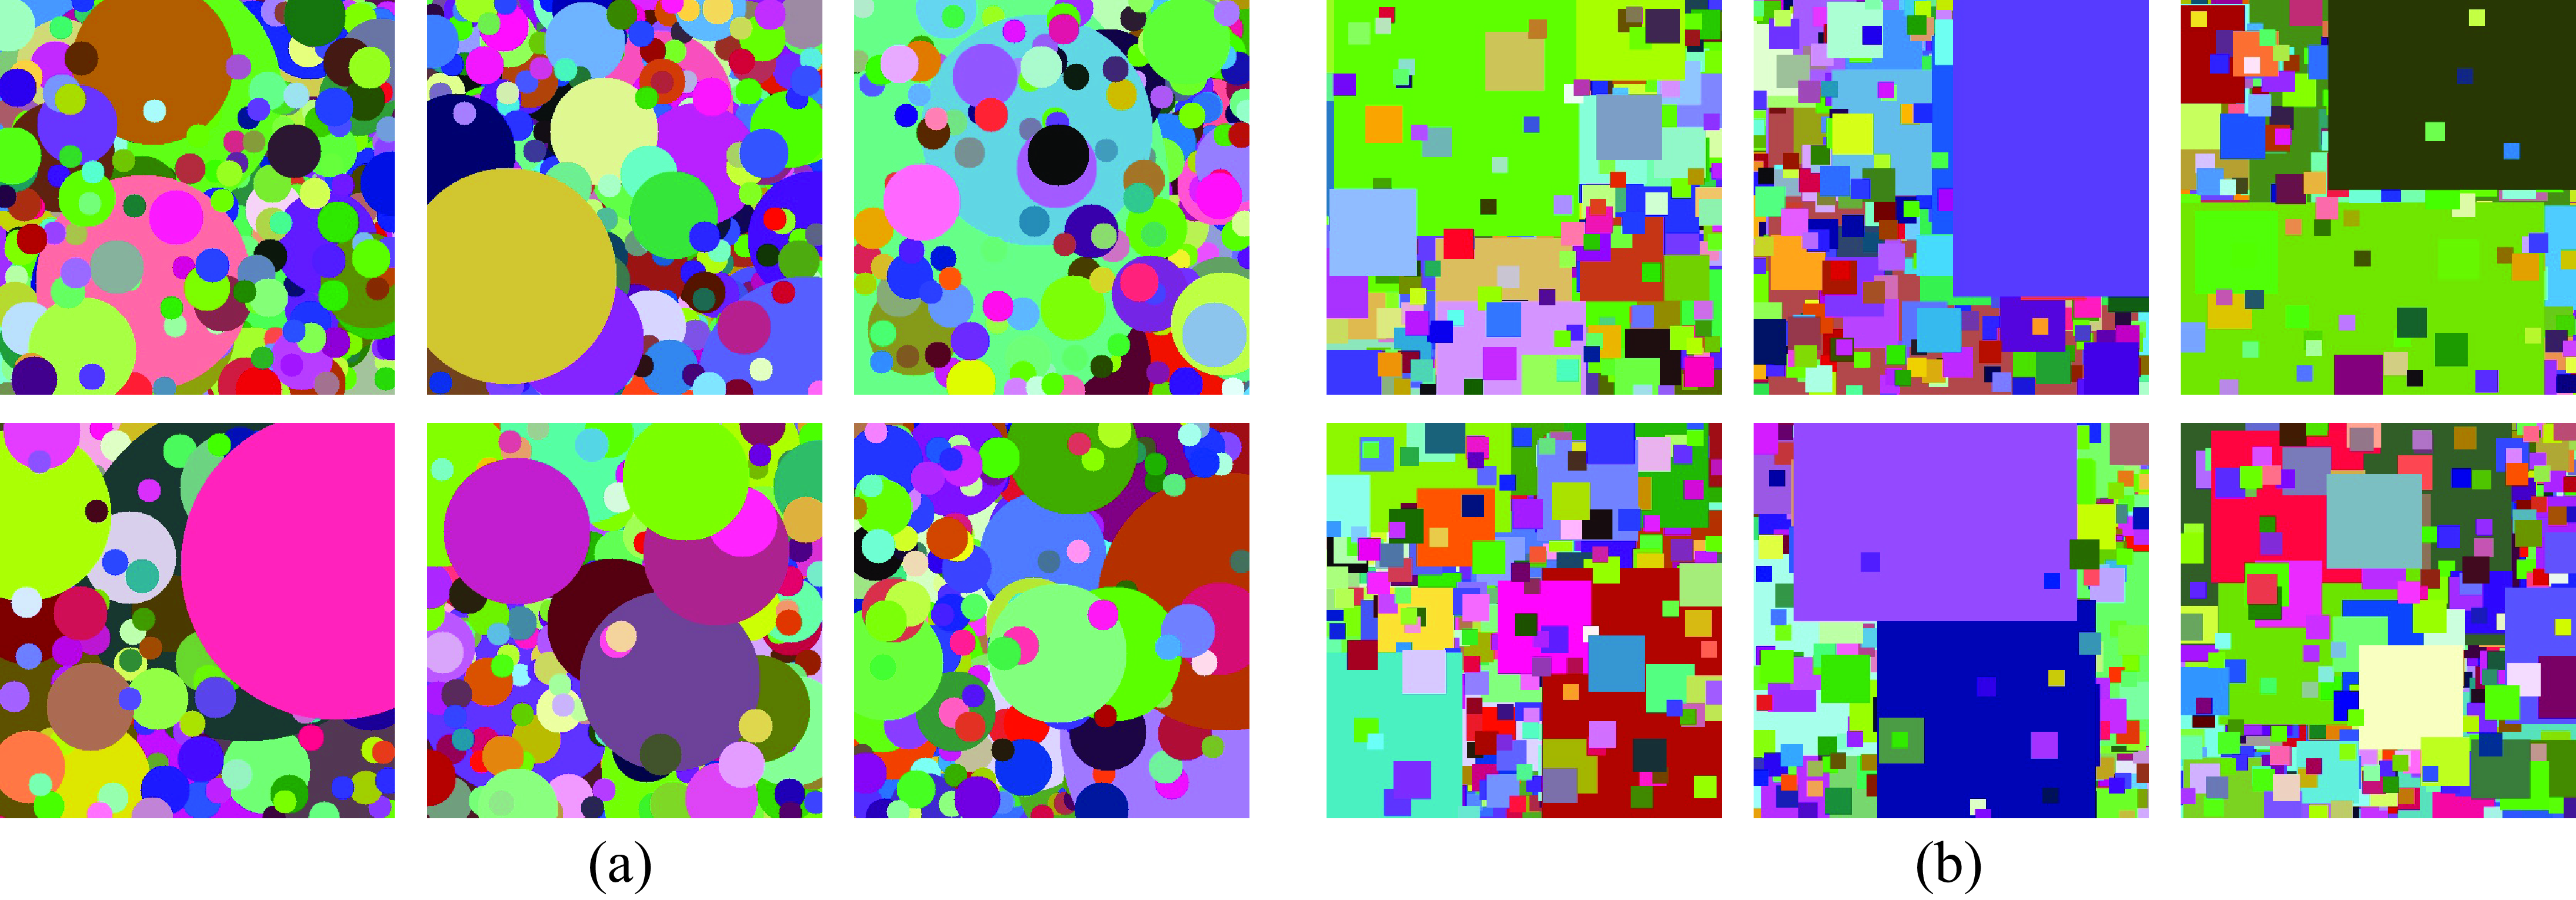
\includegraphics[width=1\linewidth]{figures/statistical_image_models/dead_leaves_squares_and_circles.eps}
} 
\caption{Images sampled from the dead leaves model, for different shapes of dead leaves. (a) Circles, and (b) Squares.
%BUILD SOME CUSTOM MADE IMAGES THAT CORRESPOND TO SOME INTERESTING VARIANTS.  For example: additive, occlusions, scale invariant and plot the measured correlation functions.
} 
\label{fig:deadleaves}
\end{figure}

The dead leaves model produces very simple images that do not look realistic, but it is useful in explaining the distribution of albedos in natural images. This model is used by the Retinex algorithm \cite{Land83} to separate an image into illumination and albedo variations, as we saw in \chap{\ref{chapter:image_derivatives}}. 
%We will see this later.

\subsection{The Power Spectrum of Natural Images}

The correlation function from \eqn{\ref{eq:correlation_between_two_pixels}} is related to the magnitude of the Fourier transform of an image. 
\marginnote{The Fourier transform of the autocorrelation of a signal is the square of magnitude of its Fourier Transform. The square of the magnitude of the FT, $\lVert \capitalimg (u,v) \rVert ^2$, is the power spectrum of a signal.}

Interestingly, the one remarkable property of most natural images is that if you take the 2D Fourier transform of an image, its magnitude falls off as a power law in frequency:
\begin{equation}
\lVert \capitalimg (u,v) \rVert \simeq \frac{1}{  w  ^ \alpha}
\label{eq:power_law_natural_images}
\end{equation}
where $w$ denotes the radial spatial frequency ($w = \sqrt{u + v}$), $\capitalimg(u,v)$ is the Fourier transform of the image $\img [n,m]$, and $\alpha \simeq 1$. And this is true for all orientations (you can think of this as taking the Fourier transform and looking at the profile of a slice that passes by the origin). 

The fact that most natural images follow \eqn{\ref{eq:power_law_natural_images}} has been the focus of an extensive literature \cite{Field1987,VANDERSCHAAF1996}, and it has been shown to be related to several properties of the early visual system \cite{Atick1990,Atick1992} which is adapted to process natural images. We will see in the next section how this model can be used to solve a number of image processing tasks.  


\Fig{\ref{fig:FT_angular_averages}} shows three natural images and the magnitude of their FT (middle row), and compares them to a random image where each pixel is independently sampled from a uniform distribution. The frequency $(0,0)$ lies in the middle of each FT. From the images in the middle row, we can see that the largest amplitudes concentrate in the low spatial frequencies for the natural images (we already discussed this in \chap{\ref{chapter:fourier_analysis}}). However, the random image has similar spectral content at all frequencies. In order to better appreciate the particular decay in the spectral amplitude with frequency, we can express the FT using polar coordinates, then calculate the average magnitude of the FT by aggregating the values over all angular directions.  The result is shown in the bottom row of \fig{\ref{fig:FT_angular_averages}}. The plot also shows three additional curves corresponding to $1/w$, $1/w^{1.5}$, and $1/w^2$. The plots are normalized to start at 1. These images have size 512$\times$512. The frequency ranges used for the plot are $w \in [20,256]$. As we can see from the middle row, there are differences on how spectral content is organized across orientations, but the decay along the radial frequency roughly follows a $1/w^{1.5}$ decay in these examples. And these property is shared across the four images despite their very distinct appearance. 


\begin{figure}
\centerline{
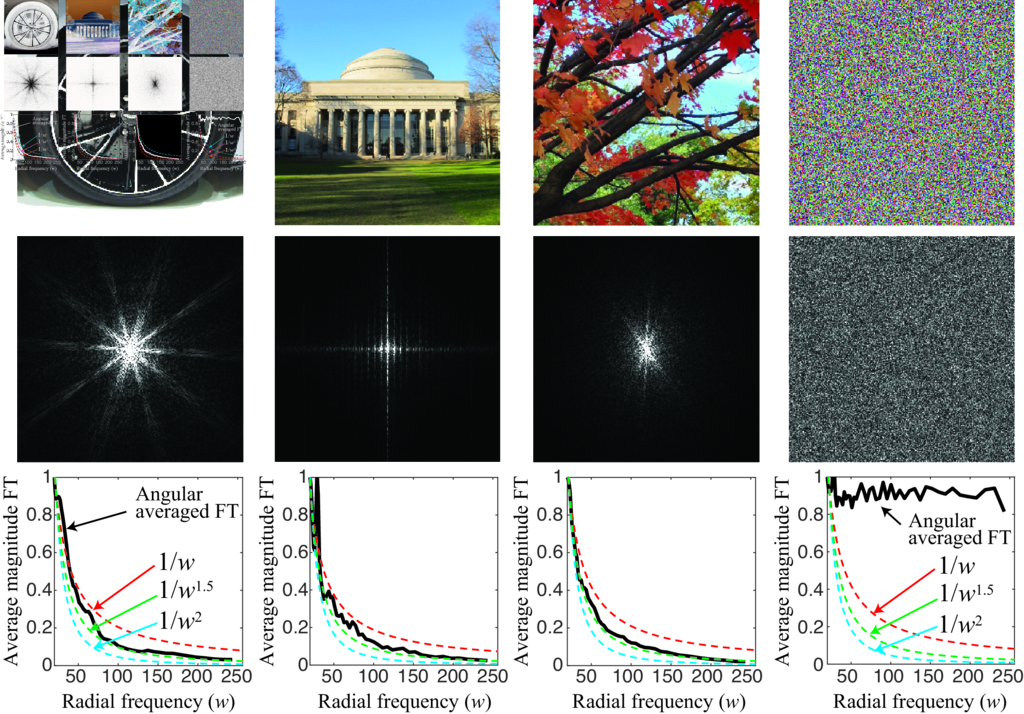
\includegraphics[width=1\linewidth]{figures/statistical_image_models/FT_power_law_angular2.eps}
} 
\caption{(top) Three natural images with size 512$\times$512 pixels, and one random image. (middle) The magnitude of their Fourier transforms (FT), images are transformed to grayscale by averaging the three color channels. (bottom) Plot of the angular average of radial sections of the FT, compared with the curves that correspond to $1/w$, $1/w^{1.5}$, and $1/w^2$, where $w$ is the radial frequency. We can see that the FT of the three natural images decays roughly with $1/w^{\alpha}$. The noise image is very different (has a flat magnitude).
} 
\label{fig:FT_angular_averages}
\end{figure}


We will now use this observation to build a better statistical model of images than using pixel histograms as we described in \sect{\ref{sec:independent_pixels}}. 

%FIGURE: noise FT and see you can see differences in the type of textures. 

\section{The Gaussian Model}

We want to write a statistical image model that takes into account the correlation statistics and the power spectrum of natural images (see \cite{Simoncelli2005} for a review). If the only constraint we have is the correlation function among image pixels, which mean that among all the possible distributions, the one that has the maximum entropy (thus, imposing the fewest other constraints) is the Gaussian distribution: 
\begin{equation}
p(\boldimg) \propto \exp \left(-\frac{1}{2} \boldimg^\transpose {\bf C}^{-1} \boldimg \right)
\label{eq:gaussianmodel}
\end{equation}
where ${\bf C}$ is the covariance matrix of all the image pixels. %Note that this model does not assume Independence across pixels anymore. This model takes into account that intensity values for different pixels are correlated as discussed in the previous sections. 
Note that this model no longer assumes independence across pixels. It accounts for the correlation of intensity values between different pixels, as discussed in previous sections. 
This model is also related to studies that use principal component analysis to study the typical components of natural images \cite{Hancock1970}. 

For stationary signals, the covariance matrix ${\bf C}$ has a circulant structure (assuming a tiling of the image) and can be diagonalized using the Fourier transform. The eigenvalues of the diagonal matrix correspond to the power (squared magnitude) of the frequency components of the Fourier transform. This is, the matrix ${\bf C}$ can be written as ${\bf C} = {\bf F}{\bf D}{\bf F}^\transpose$. Where ${\bf F}$ is the matrix that contains the Fourier basis, as seen in \chap{\ref{chapter:fourier_analysis}}, and the diagonal matrix ${\bf D}$ has, along the diagonal, the values $1/ w  ^\alpha$ for all radial frequencies $w$. The value of $\alpha$ can be set to a fix value of 1.5. 

% http://ee.stanford.edu/~gray/toeplitz.eps


%The gaussian model is the result of making a number of assumptions about images:
%
%\begin{itemize}
%\item Stationarity
%\item Scale invariance
%\end{itemize}


\subsection{Sampling Images}

Once a distribution is defined, we can use it to sample new images. First we need to specify the parameters of the distribution. In this case, we need to specify the covariance matrix ${\bf C}$. \Fig{\ref{fig:figure_samples_1_over_f}} shows the results of sampling images using the $1/ w^\alpha$ model to fill the diagonal values of the matrix ${\bf D}$. These images are generated by making an image with a random phase and with a magnitude of the power spectrum following $1/(1+w ^\alpha)$ with $\alpha=1.5$. We add 1 to the denominator term to avoid division by zero. The bottom row of \fig{\ref{fig:figure_samples_1_over_f}} generates color images by sampling each color channel independently. 



\begin{figure}
\centerline{
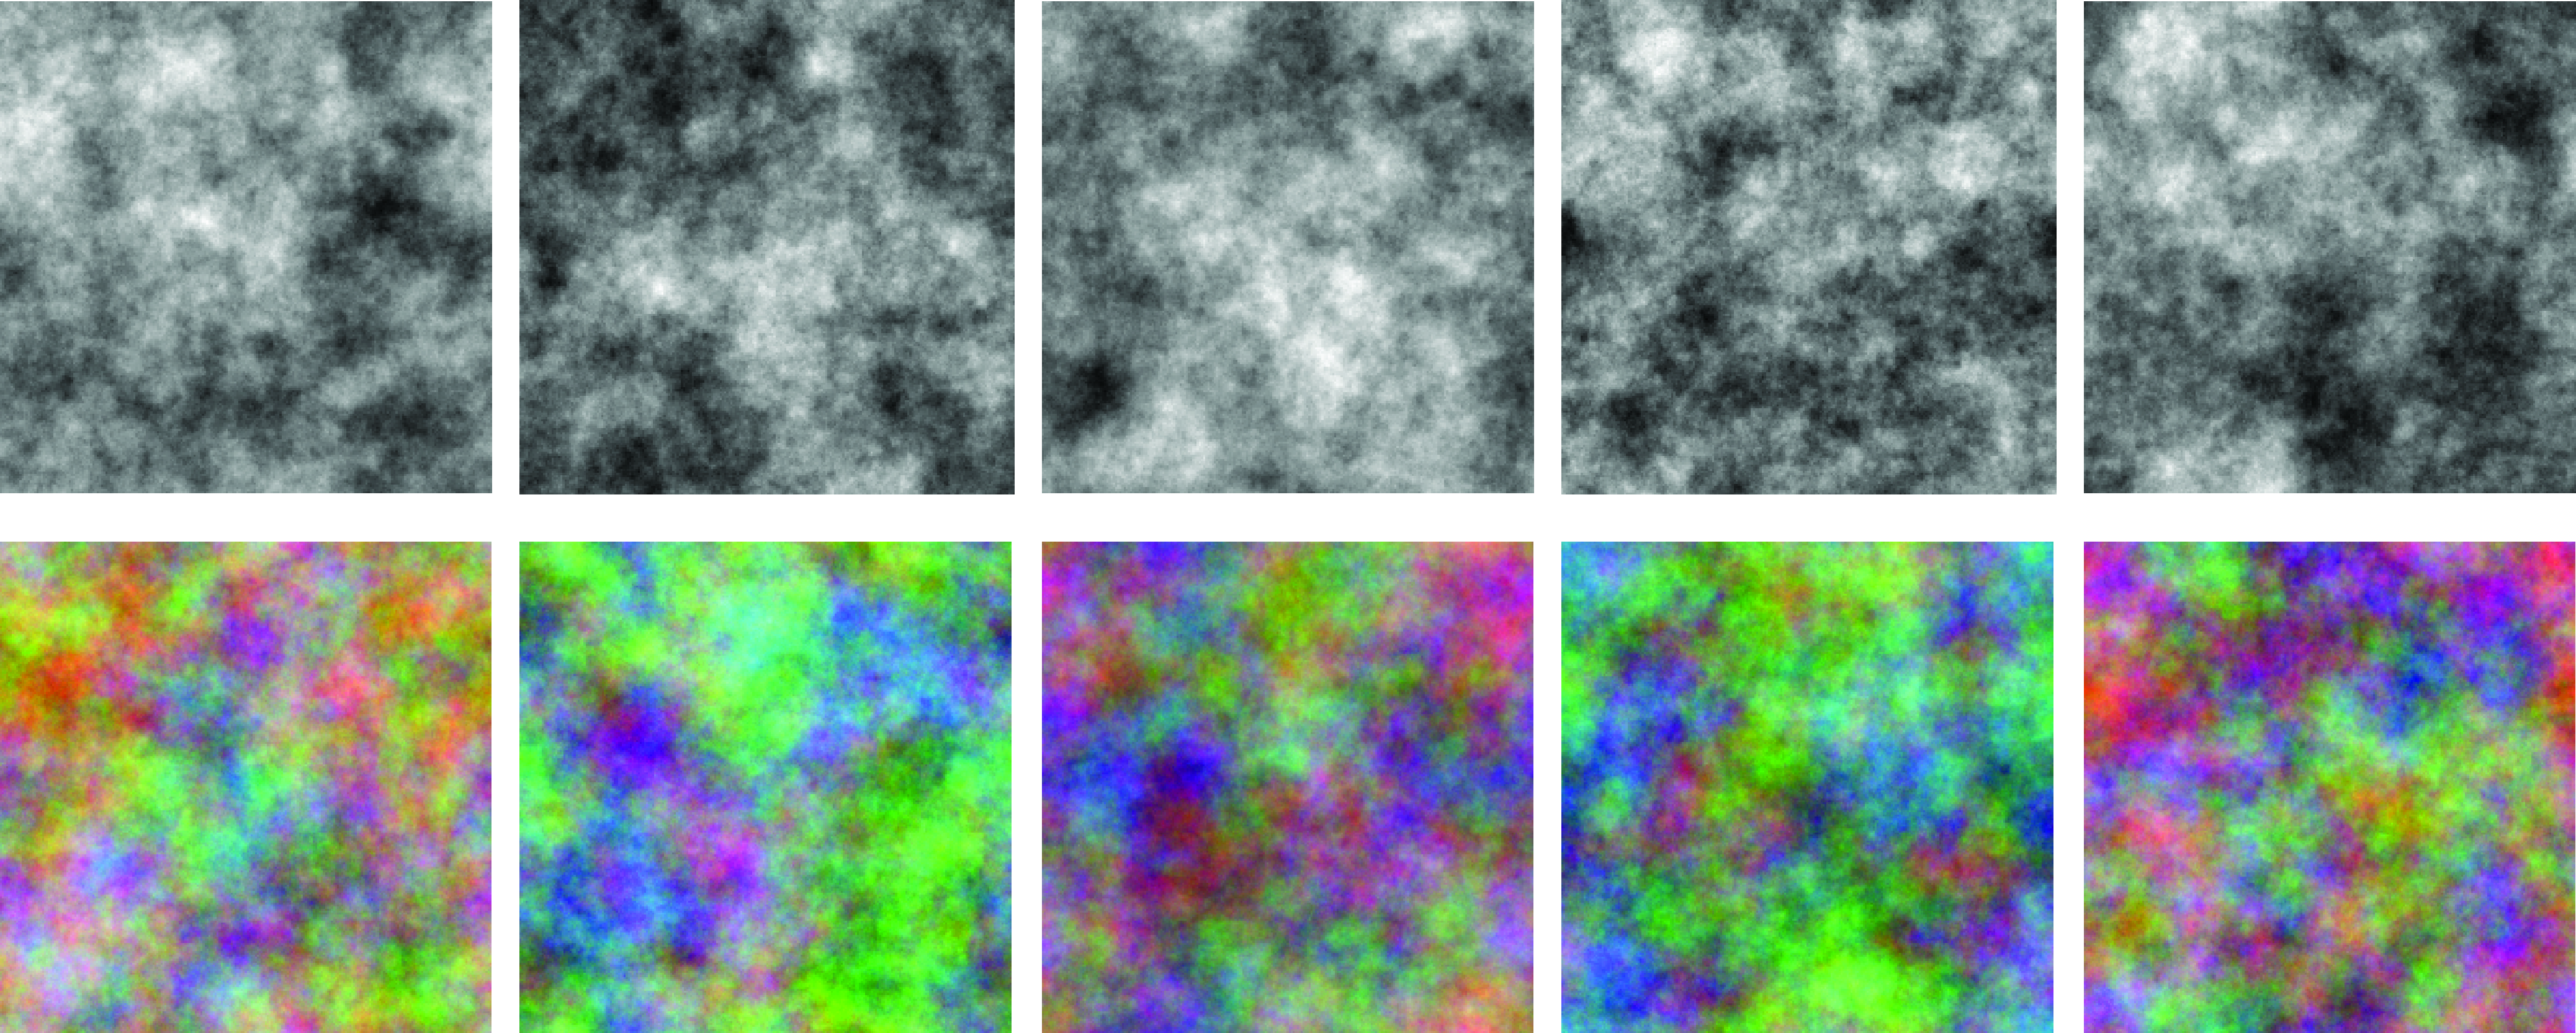
\includegraphics[width=1\linewidth]{figures/statistical_image_models/figure_samples_1_over_f.eps}
} 
\caption{(top) Images are generated by making an image with a random phase and with a magnitude of the power spectrum following $1/ (1+w ^\alpha)$ with $\alpha=1.5$. (bottom) Same generative process applied to each color channel independently. The generated images look like clouds.
} 
\label{fig:figure_samples_1_over_f}
\end{figure}




We can also sample new images by matching the parameter of individual natural images. \Fig{\ref{fig:magFTMatch}} shows four examples. To process color images, we first look for a color space that decorrelates color information for each image. This can be done by applying principal component analysis (PCA) to the three color channels. This results in a 3$\times$3 matrix that will produce three new channels that are decorrelated. Then, for each channel, we compute the FT and keep the magnitude and replace the phase with random noise. We finally compute the new generated imaged by doing the inverse FT and applying the inverse of the PCA matrix in order to return to the original color space. This results in images that keep a similar color distribution than the inputs. 


%\Fig{\ref{fig:synthClouds}} shows an example of an image of clouds and the magnitude of its Fourier transform. A sample of the distribution can be obtained by filtering white Gaussian noise using the image magnitude as a filter. It can also be obtained by randomizing the phase, while keeping the magnitude of the Fourier transform the same. 
%As shown in \fig{\ref{fig:magFTMatch}}, samples from this model still roughly looks like clouds.


\begin{figure}
\centerline{
\includegraphics[width=1\linewidth]{figures/statistical_image_models/4_examples_images_color_FT.eps}
} 
\caption{Examples of images and random samples with the same magnitude of the FT of the corresponding image. We use PCA in color space to find decorrelated color components. Then, each decorrelated color channel is sampled independently and the final image is created by returning to the original color space. Only the image with clouds (b) has some visual similarity with the randomly sampled image.}
\label{fig:magFTMatch}
\end{figure}


%\begin{figure}[t]
%\centerline{
%\includegraphics[width=1\linewidth]{figures/statistical_image_models/synthClouds.eps}
%} 
%\caption{Left: cloud image, Center: magnitude of its Fourier transform, Right:  random draw from the same Gaussian image model, obtained by randomizing the phase, while keeping the magnitude of the Fourier transform the same.  The result still roughly looks like clouds.}
%\label{fig:synthClouds}
%\end{figure}


As shown in \fig{\ref{fig:magFTMatch}}, when fitting the Gaussian model to different real images, and then sampling from it, the result is always an image that looks like cloudy noise regardless of the image content. However, a few attributes of the original image are preserved including the size of the details present in the image and the dominant orientations. 

\begin{comment}
\begin{figure}[t]
\centerline{
\sublabelnp{(a)}
{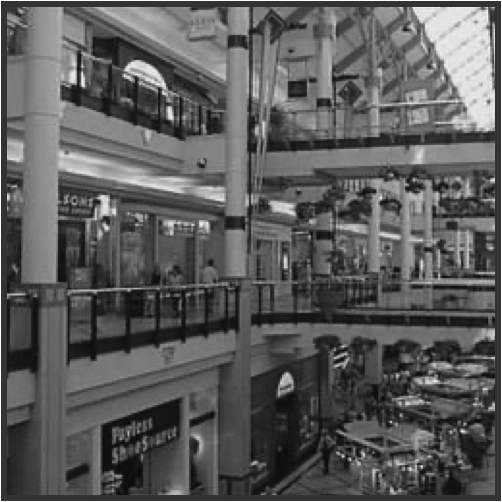
\includegraphics[width=0.3\linewidth]{figures/statistical_image_models/photo1.jpg}}
\sublabelnp{(b)}{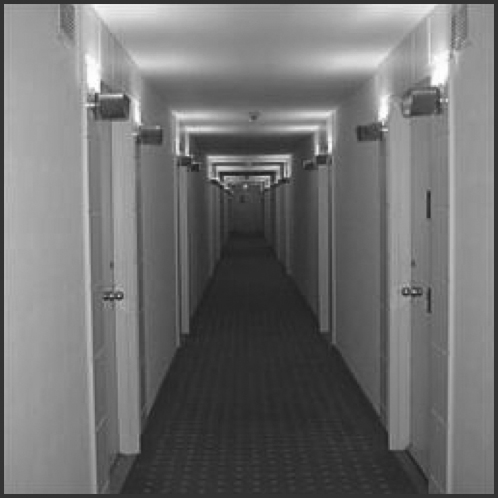
\includegraphics[width=0.3\linewidth]{figures/statistical_image_models/photo2.jpg}}
\sublabelnp{(c)}{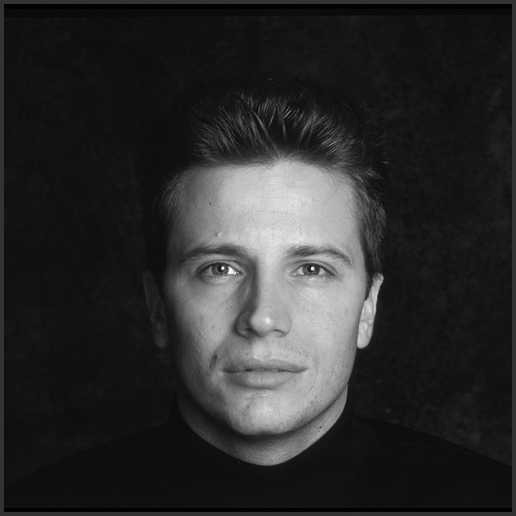
\includegraphics[width=0.3\linewidth]{figures/statistical_image_models/photo3.jpg}}
}
\centerline{
\sublabelnp{(d)}
{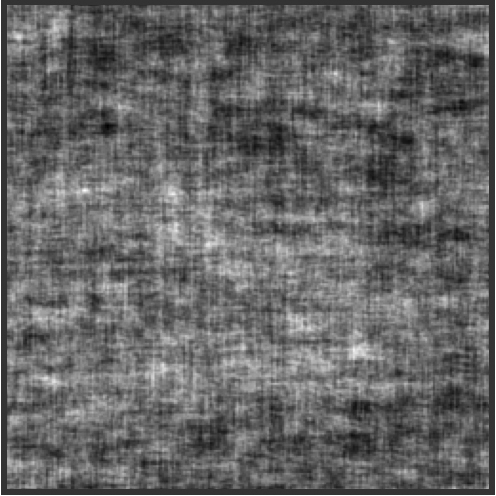
\includegraphics[width=0.3\linewidth]{figures/statistical_image_models/photo1mush.jpg}}
\sublabelnp{(e)}{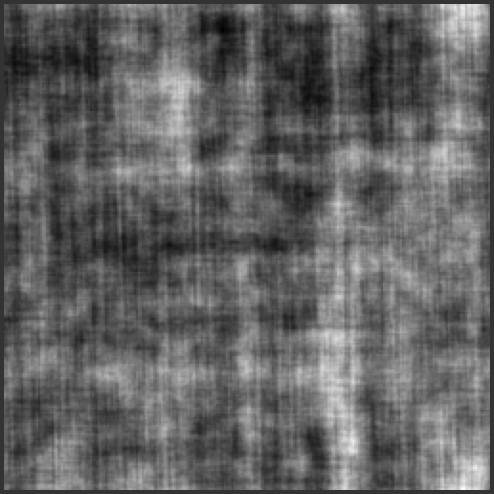
\includegraphics[width=0.3\linewidth]{figures/statistical_image_models/photo2mush.jpg}}
\sublabelnp{(f)}{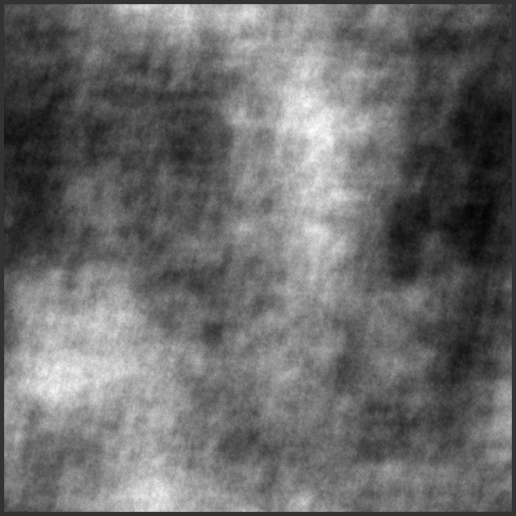
\includegraphics[width=0.3\linewidth]{figures/statistical_image_models/photo3mush.jpg}}
}
\caption{Top row, (a), (b), (c):  three images. Bottom row (d), (e), (f): Images with identical covariance structure as the image above it, made by randomizing the phases of the sinusoidal components of each image.  Under the Gaussian model, each image in the top row is equally probable as the image below it.
}
\label{fig:GaussModelexamples}
\end{figure}
\end{comment}

\Fig{\ref{fig:hair}} shows an example image where the sample from its Gaussian model produces a similar image,  due to the strong oriented pattern present in the image. In this example, the input image is mostly one-dimensional (1D) as most of the variations occur across one orientation being constant along the perpendicular direction. This structure can be captured by the magnitude of the Fourier transform of the image. 

\begin{figure}[t]
\centerline{
\sublabelnp{(a)}
{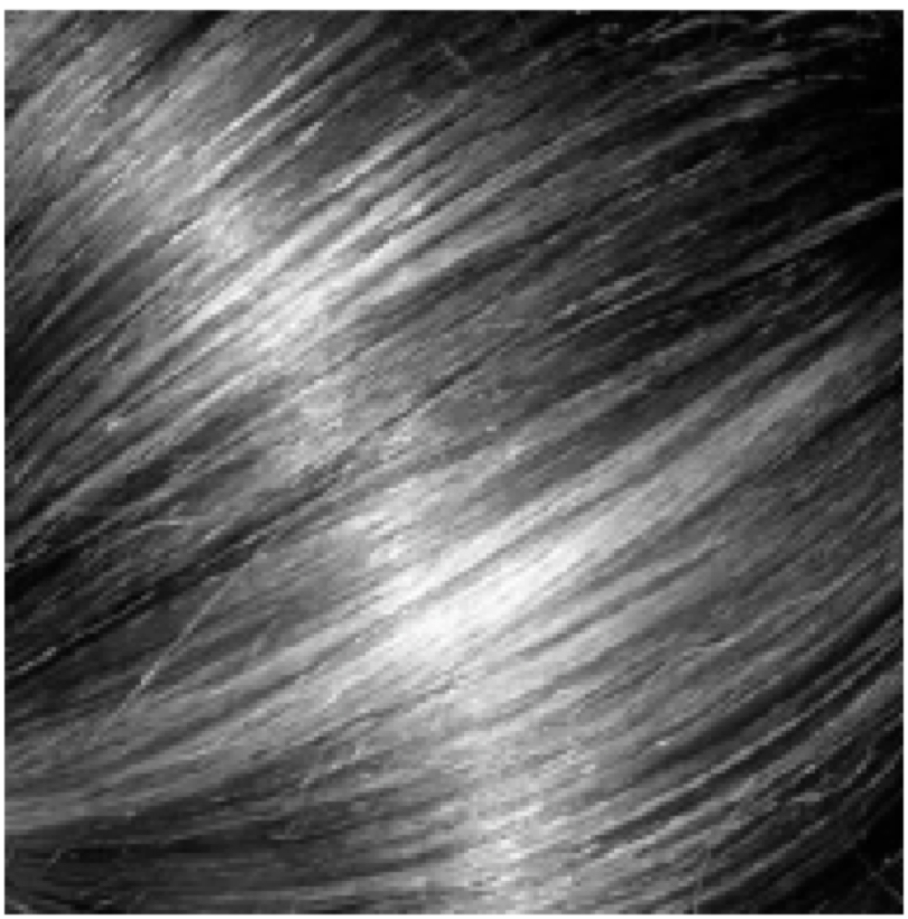
\includegraphics[width=0.4\linewidth]{figures/statistical_image_models/hair1.pdf}}
\sublabelnp{(b)}{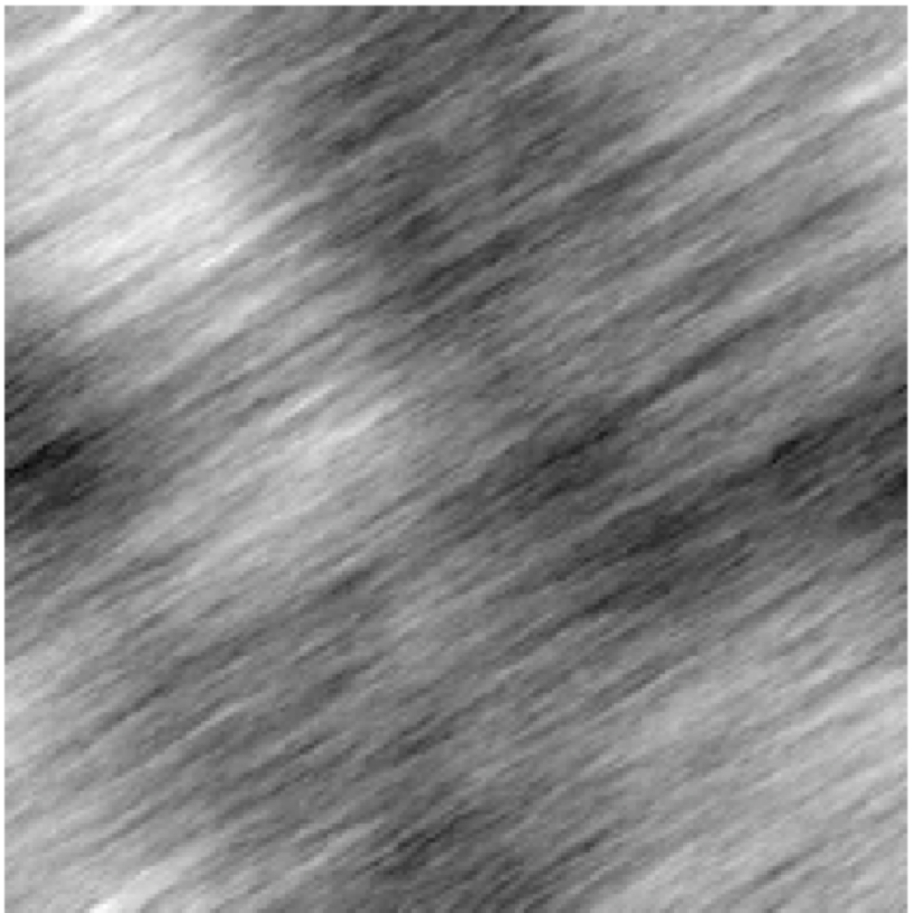
\includegraphics[width=0.4\linewidth]{figures/statistical_image_models/hair2.pdf}}
}
\caption{(a) Photograph of hair.  (b) Random draw of Gaussian image model using covariance matrix fit from (a).  For this unusual image, the model works well, but this is an exception for the Gaussian image model.}
\label{fig:hair}
\end{figure}

%
%\begin{figure}[htpb]
%\centerline{
%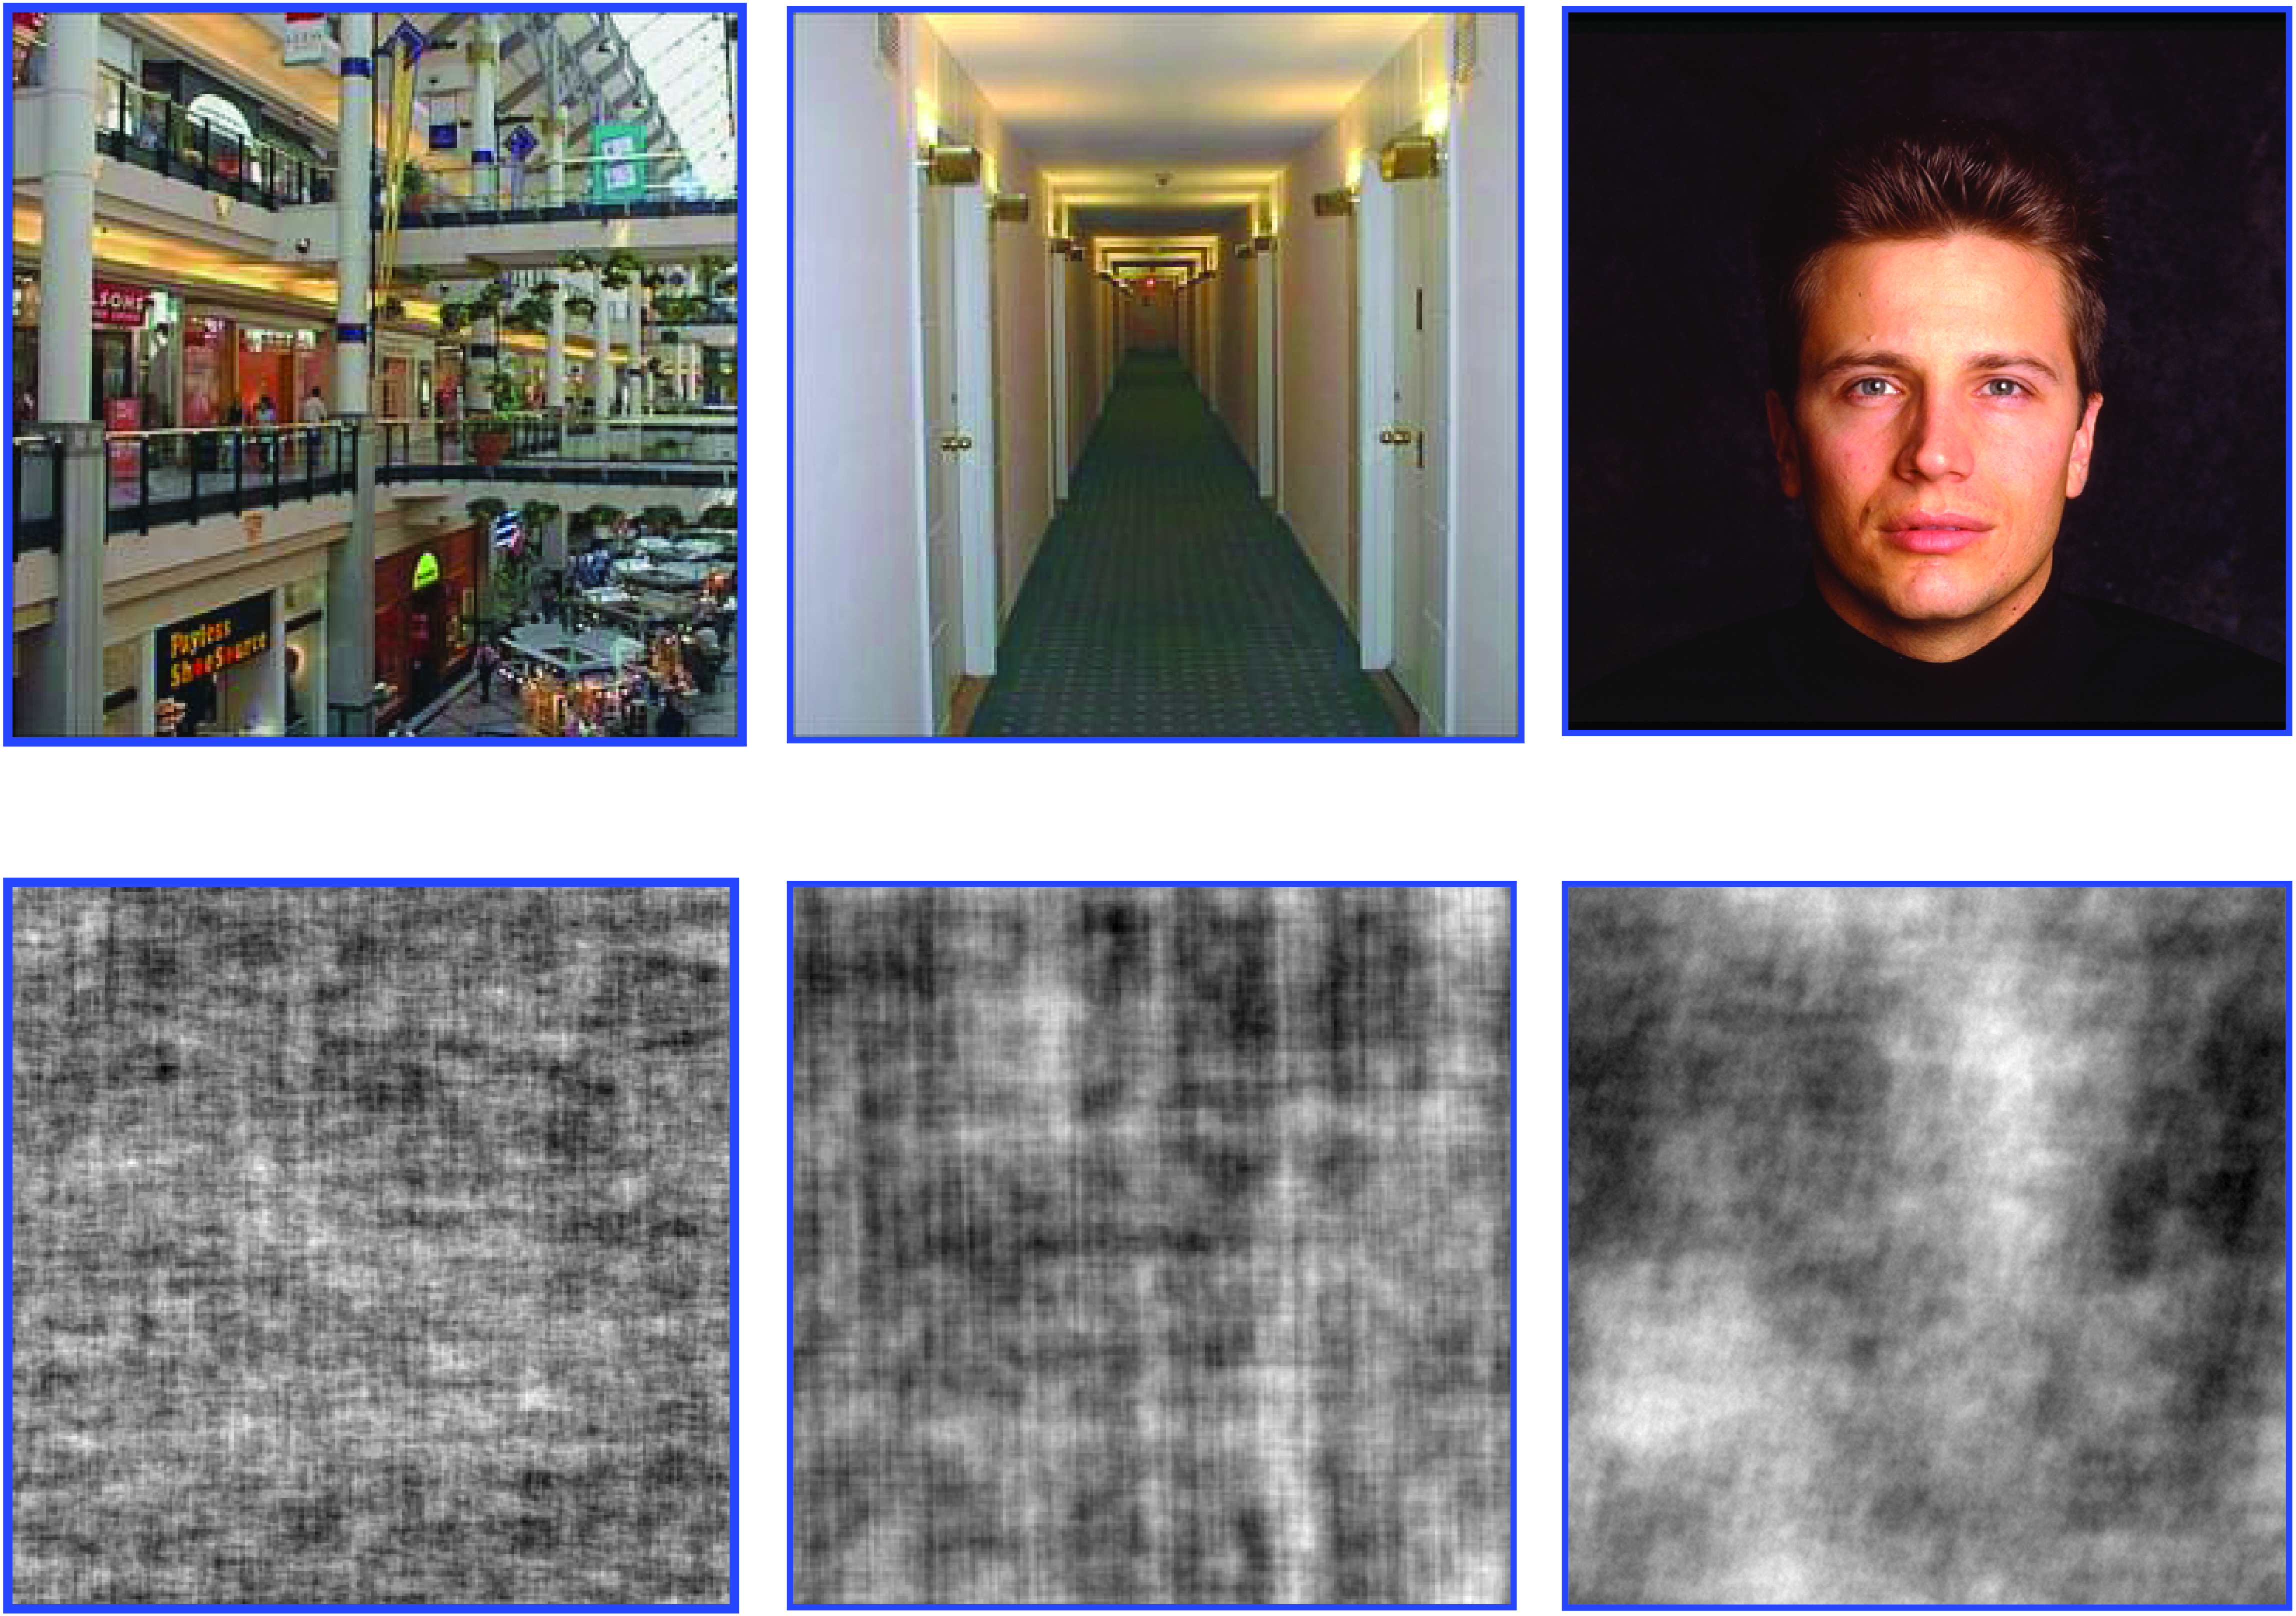
\includegraphics[width=1\linewidth]{figures/statistical_image_models/phaserandomization.eps}
%} 
%\caption{BUILD MORE DISTINCT IMAGES: face, beach, forests with vertical trees.} 
%\label{fig:phaserandomization}
%\end{figure}
%
%


The Gaussian image model, despite being very simple, can be used to study some image processing tasks, including image denoising, which we will discuss next.

\marginnote{Devising processes that generate realistic textures has a long history and many applications in the movie industry. One example is Perlin noise developed by Ken Perlin in 1985. In the rest of this book, we will study in depth the image generation problem when talking about generative models.}\index{Perlin noise}

\subsection{Image Denoising under the Gaussian Model: Wiener Filter}
\label{sec:image_denoising_gaussian_model}

As an example of how to use image priors for vision tasks, we will study how to do image denoising using the prior on the structure of the correlation of natural images. In this problem, we observe a noisy image $\boldimg_g$ corrupted with white Gaussian noise: 
\begin{equation}
\img_g[n, m] = \img[n, m] + g[n, m]
\end{equation}
The goal is to recover the uncorrupted image $\img [n,m]$. The noise $g[m, n]$ is white Gaussian noise with variance $\sigma_g^2$. The denoising problem can be formulated as finding the $\img [n,m]$ that maximizes the probability of the uncorrupted image, $\boldimg_g$, called the maximum a posteriori, or MAP, estimate:
\begin{equation}
\max_{\boldimg} p(\boldimg \given \boldimg_g) 
\end{equation}

In these equations we write the image as a column vector $\boldimg$. This posterior density can be written as:
\begin{equation}
\max_{\boldimg} p({\boldimg} \given {\boldimg}_g) = \max_{\boldimg} p({\boldimg}_g \given {\boldimg}) p({\boldimg})
\end{equation}
where the likelihood and prior functions are:
\begin{eqnarray}
p({\boldimg}_g \given {\boldimg}) & \propto & \exp( - \left| {\boldimg}_g - {\boldimg} \right| ^2 / \sigma_g^2) \\ 
%\end{equation}
%and the prior:
%\begin{equation}
p({\boldimg}) & \propto & \exp \left(-\frac{1}{2} {\boldimg}^T {\bf C}^{-1} {\boldimg} \right)
\end{eqnarray}

The solution to this problem can be obtained in closed form:
\begin{equation}
{\boldimg} = {\bf C} \left( {\bf C} + \sigma_g^2   \mathbf{I} \right)^{-1} {\boldimg}_g
\end{equation}
This is just a linear operation. It can also be written in the Fourier domain as:
\begin{equation}
\boldcapitalimg(v) = \frac{A/|v|^{2\alpha}}{A/|v|^{2\alpha} + \sigma_g^2} \boldcapitalimg_g(v) 
\end{equation}

\Fig{\ref{fig:denoisingGaussianModel}} shows the result of using the Gaussian image model for image denoising. Although there is a certain amount of noise reduction, the result is far from satisfactory. The Gaussian image model fails to capture the properties that make a natural image look real. 

\begin{figure}[t]
\centerline{
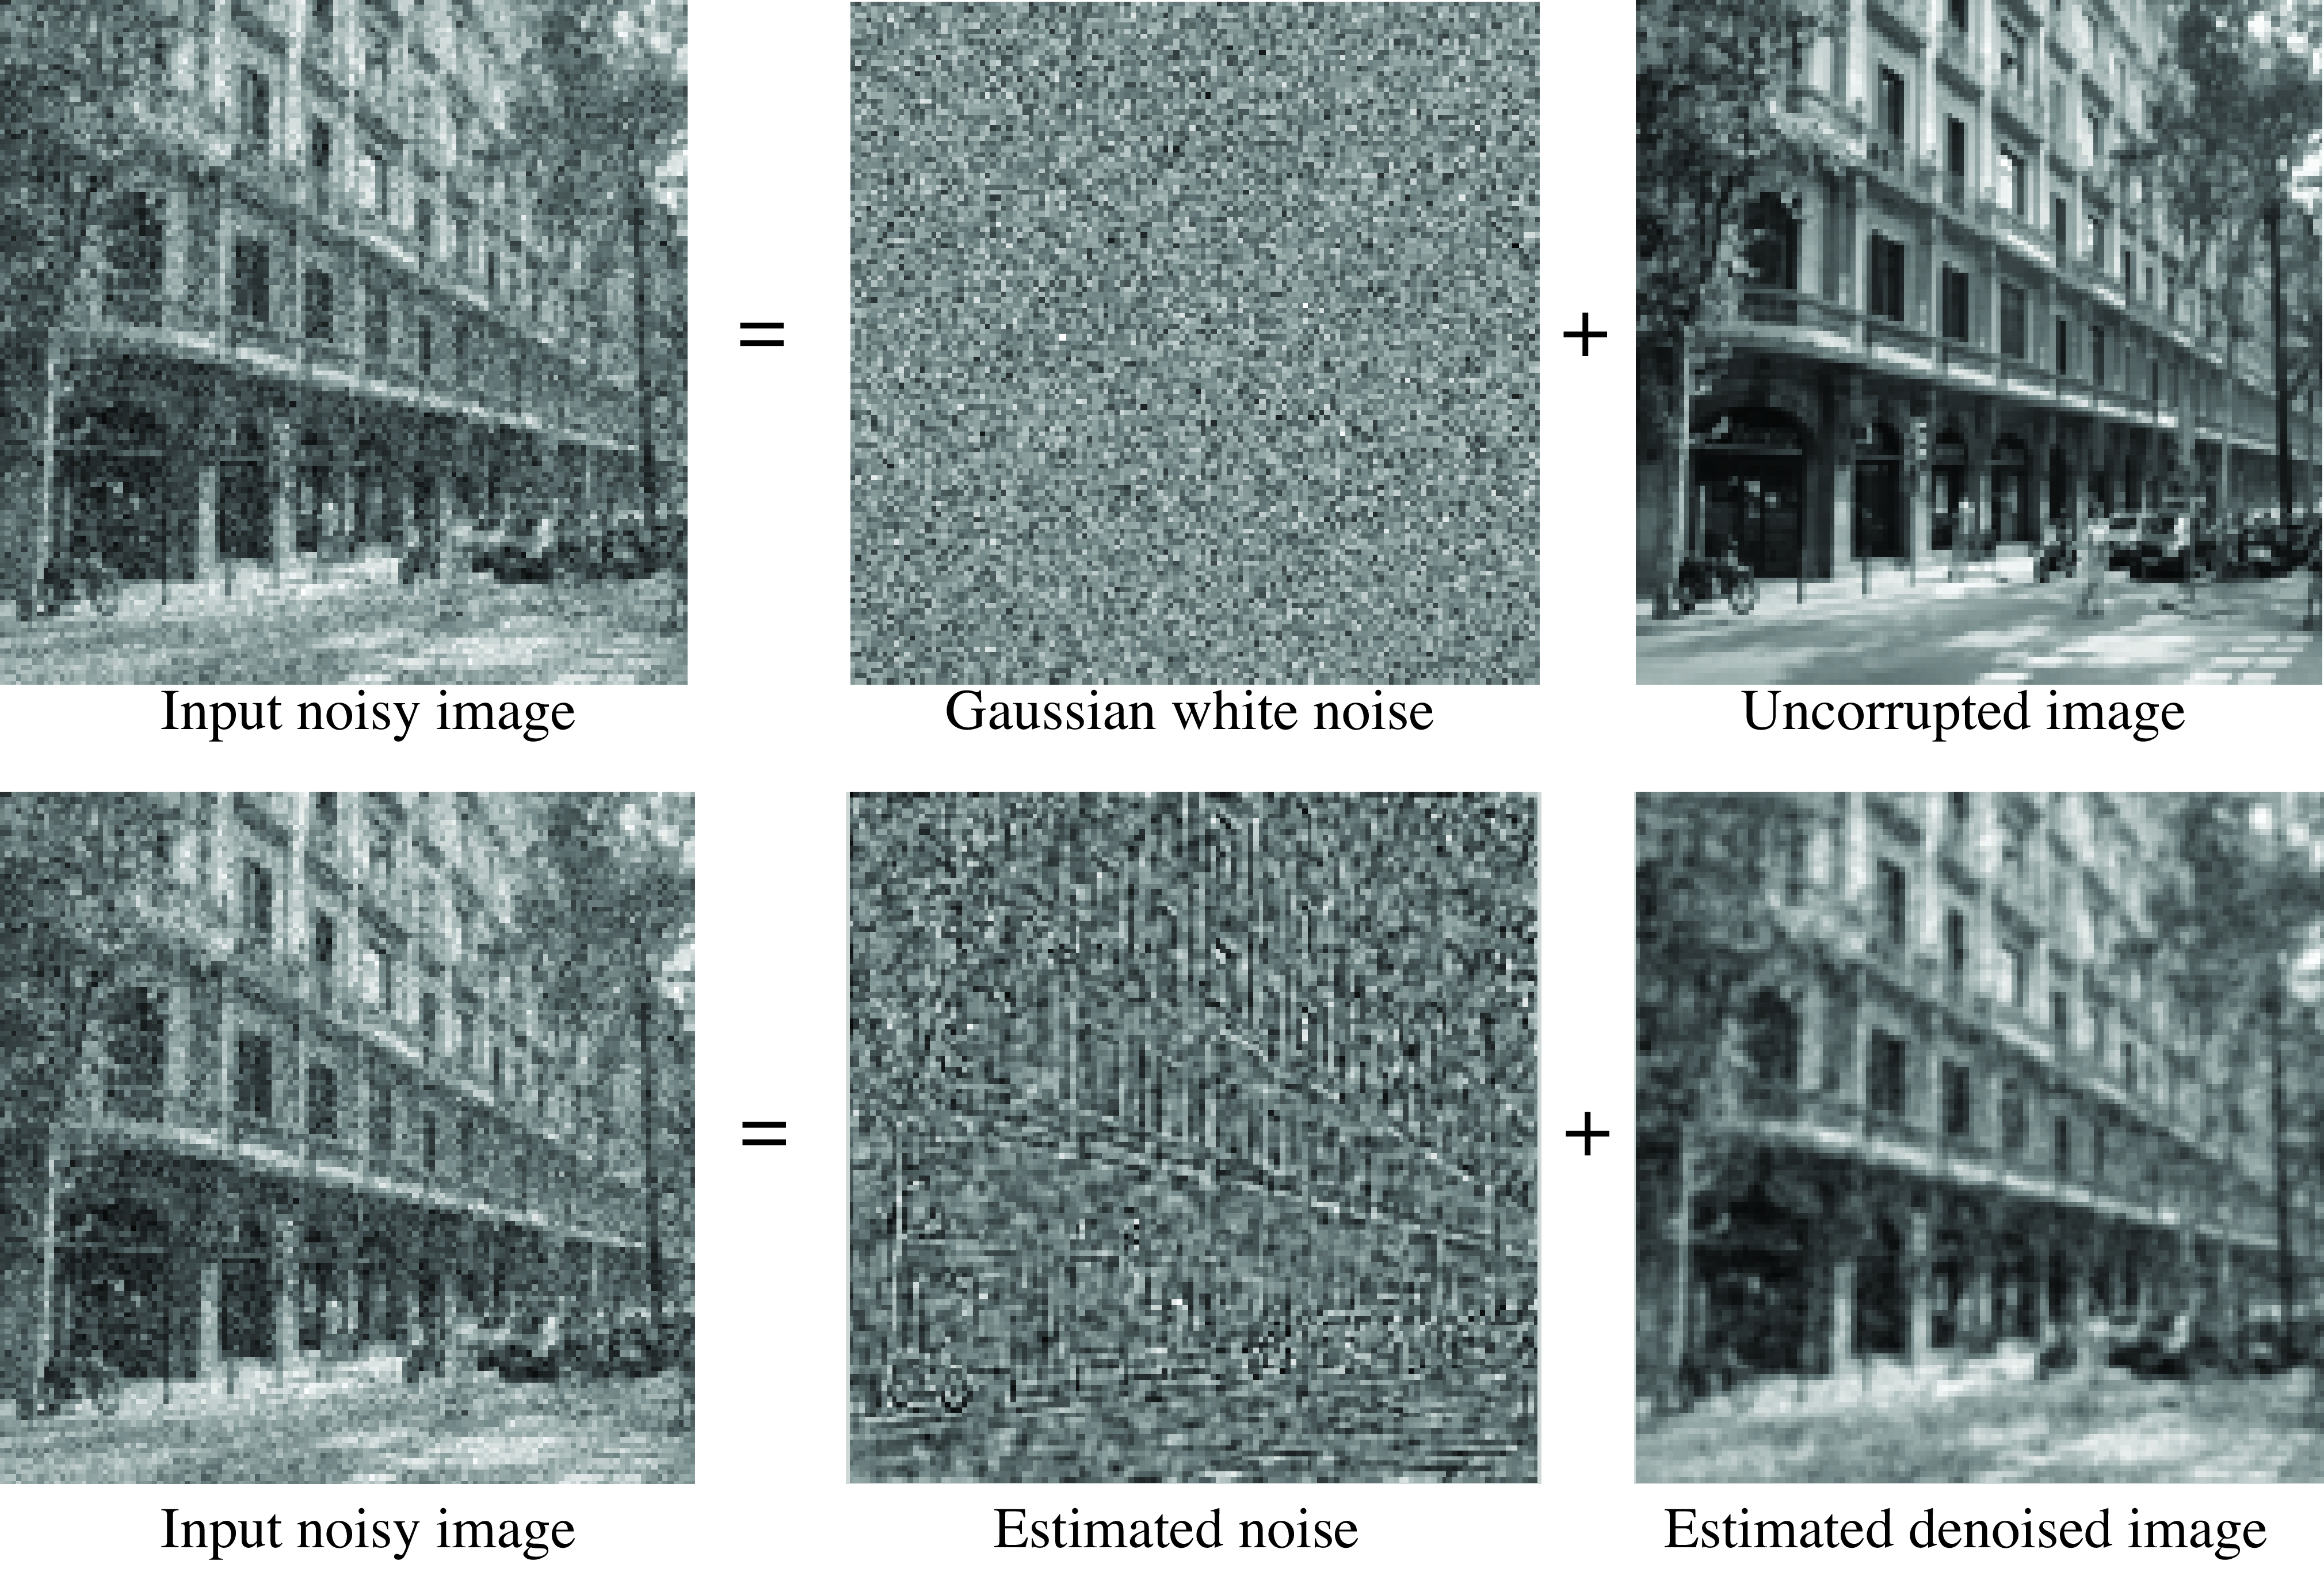
\includegraphics[width=1\linewidth]{figures/statistical_image_models/denoisingGaussianModel.eps}
} 
\caption{(Top row) Ground truth decomposition of image into Gaussian white noise and the image, uncorrupted by noise.  (bottom row) Gaussian image model denoising results.  Note that the estimated noise image shows residual spatial structure from the original image.} 
\label{fig:denoisingGaussianModel}
\end{figure}






%As a representation, the fourier transform makes explicit the dominant image orientations, the image scales, periodic patterns, ...


%FIGURE: stats for man-made vs. natural. Average spectrum. Explain phase is great to reconstruct image, but the magnitude, as a representation makes information explicit.

%Atick model of early visual system as a whitening filter.

%Denoising

%
%\subsubsection{Decorrelating image pixels}
%
%If the Gaussian model was an accurate model of images, then we could use it to find independent components of images by decorrelating image pixels. In fact, a number of models of the early visual system have hypothesized that one of the functions of the retina is to decorrelate pixel values.
%
%Maybe the retina does a bit of Wiener denoting and whitening. See figure on CSF.
%
%%\begin{figure}[htpb]
%%\centerline{
%%\includegraphics[width=1\linewidth]{figures/statistical_image_models/whitening.eps}
%%} 
%%\caption{BUILD SOME CUSTOM MADE IMAGES of the CSF.} 
%%\label{fig:whitening}
%%\end{figure}
%
%
%
%
%
%\subsubsection{Image deblurring}
%
%If an image is blurred with a Gaussian filter of unknown variance, we can try to estimate the parameter of the gaussian blurring filter by looking at the 
%\begin{equation}
%\log(\imgfft) \simeq K - \alpha \log(| v |)  -| v |^2/\sigma^2
%\end{equation}
%
%From this equation, one can try to estimate the parameters of the gaussian blurring filter.  
%
%%USE THIS PROBLEM TO ILLUSTRATE THE LIMITATIONS OF THE GAUSSIAN MODEL.
%
%% UNIFY NOTATION WITH FOURIER TRANSFORMS
%
\section{The Wavelet Marginal Model}

As we showed previously, sampling from a Gaussian prior model generates images of clouds. Although the Gaussian prior does not give any image  zero probability (i.e., by sampling for a very long time it is not impossible to sample the Mona Lisa), the most typical images under this prior look like clouds. 

The Gaussian model captures the fact that pixel values are correlated and that such correlation decreases with distance. However, it fails to capture other very important properties of images, such as flat regions, edges, and lines.  Here, we extend the Gaussian model in two ways.  (1) We will use localized filters instead of sinusoids (i.e., Fourier basis) that span the entire image, as in the power spectrum model used in the previous section.  This helps to capture local structure such as lines and edges. (2) Instead of characterizing the outputs of those filters by a single number (e.g., the mean power), we measure the histogram shape of all the filter responses. 
%We will ... ?

In the 1980s, a number of papers noticed a remarkable property of images: when filtering images with band-pass filters (i.e, image derivatives, Gabor filters, etc.) the output had a non-Gaussian distribution \cite{Daugman1989,Field1987}.
%Field (1987) and Daugman (1989)
%Daugman JG. 1989. Entropy reduction and decorrelation in visual coding by oriented neural receptive fields. IEEE Trans. Biomed. Eng. 36(1):107–14
%Field DJ. 1987. Relations between the statistics of natural images and the response properties of cortical cells. J. Opt. Soc. Am. A 4(12):2379–94
%https://www.cns.nyu.edu/pub/eero/simoncelli01-reprint.pdf
\Fig{\ref{fig:derivativeshist}} shows the histogram of the input image and the histogram of the output of applying the filters $\left[-1,1\right]$ and $\left[-1,1\right]^\transpose$.

\begin{comment}
\begin{figure}
    \centering
    \begin{subfigure}{0.3\textwidth}
        \centering
        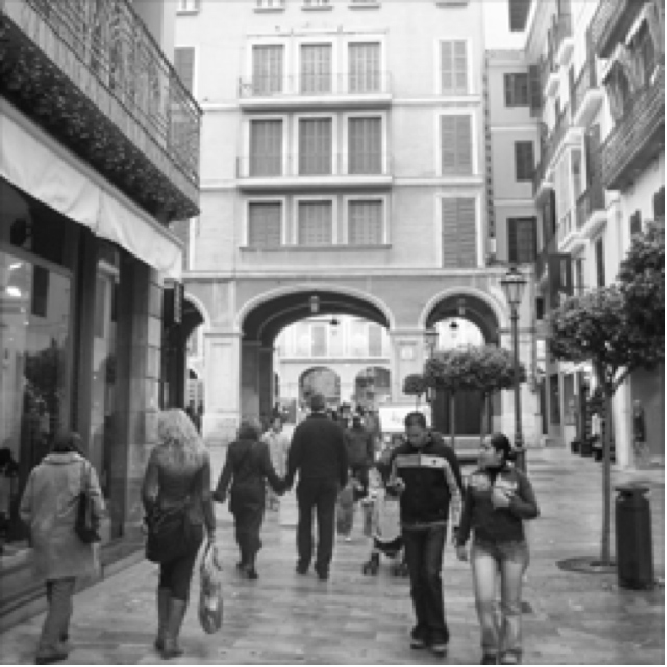
\includegraphics[width=\textwidth]{figures/statistical_image_models/spain_image.pdf}
    \end{subfigure}
    \begin{subfigure}{0.3\textwidth}
        \centering
        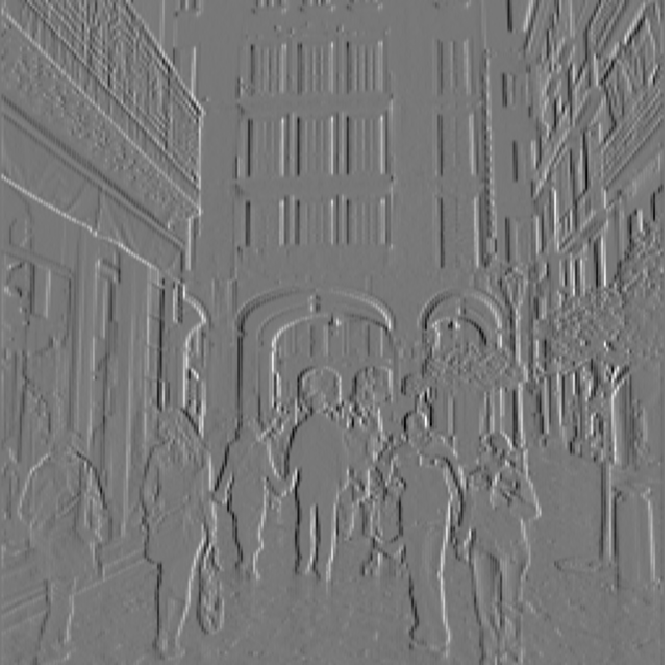
\includegraphics[width=\textwidth]{figures/statistical_image_models/spain_dx.pdf}
    \end{subfigure}
    \begin{subfigure}{0.3\textwidth}
        \centering
        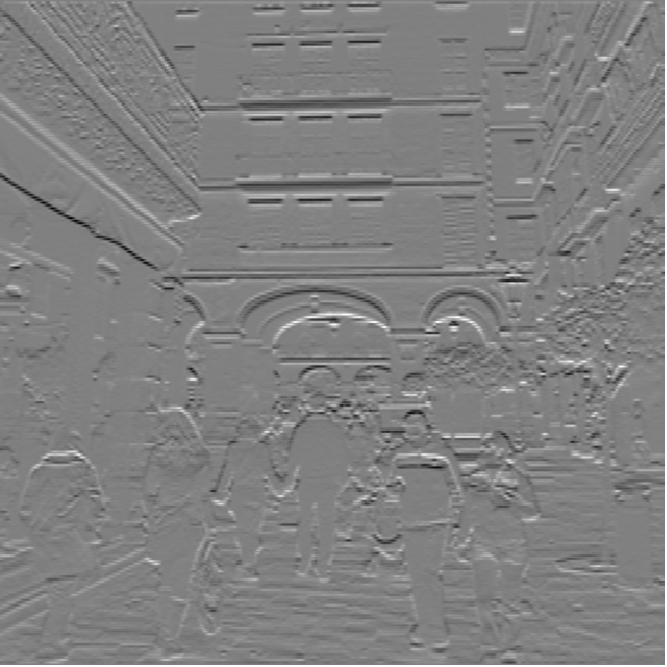
\includegraphics[width=\textwidth]{figures/statistical_image_models/spain_dy.pdf}
    \end{subfigure}
    
    \begin{subfigure}{0.3\textwidth}
        \centering
        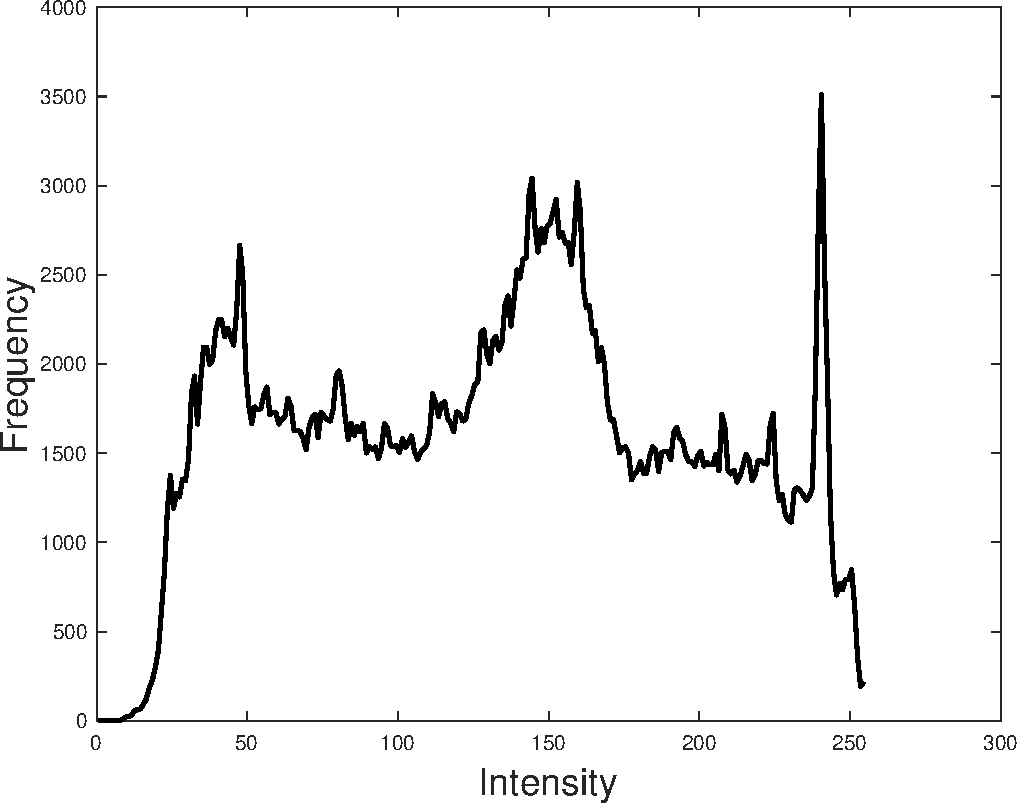
\includegraphics[width=\textwidth]{figures/statistical_image_models/spain_histogram.pdf}
    \end{subfigure}
    \begin{subfigure}{0.3\textwidth}
        \centering
        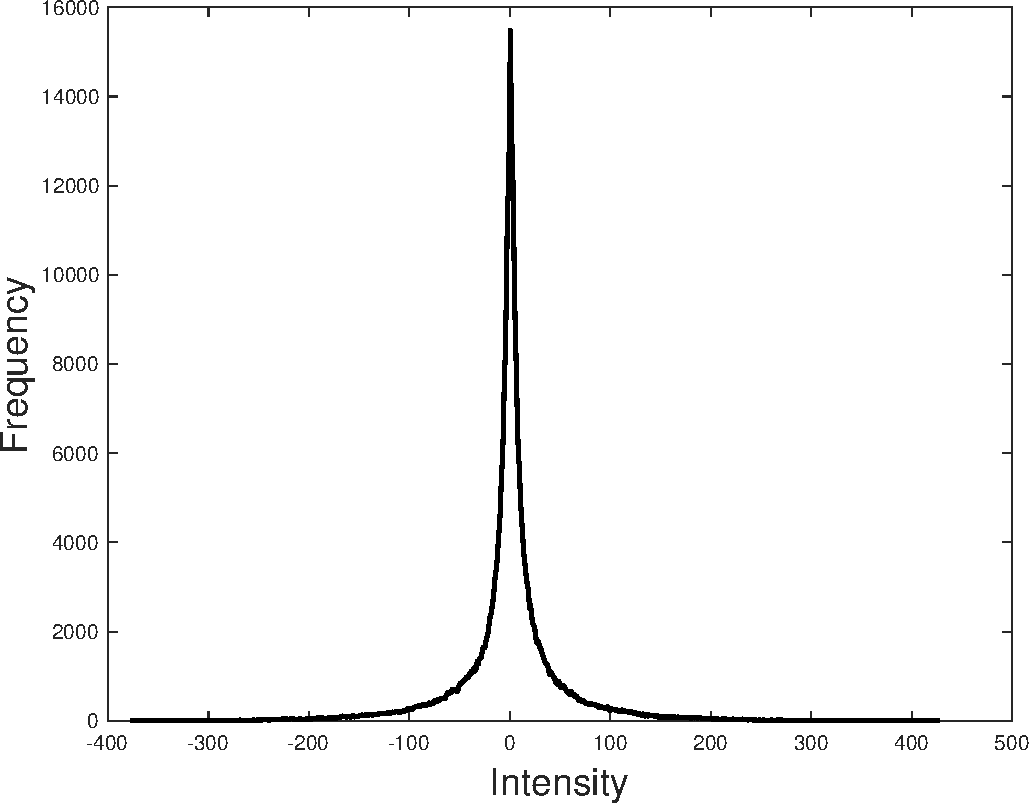
\includegraphics[width=\textwidth]{figures/statistical_image_models/spain_dx_histogram.pdf}
    \end{subfigure}
    \begin{subfigure}{0.3\textwidth}
        \centering
        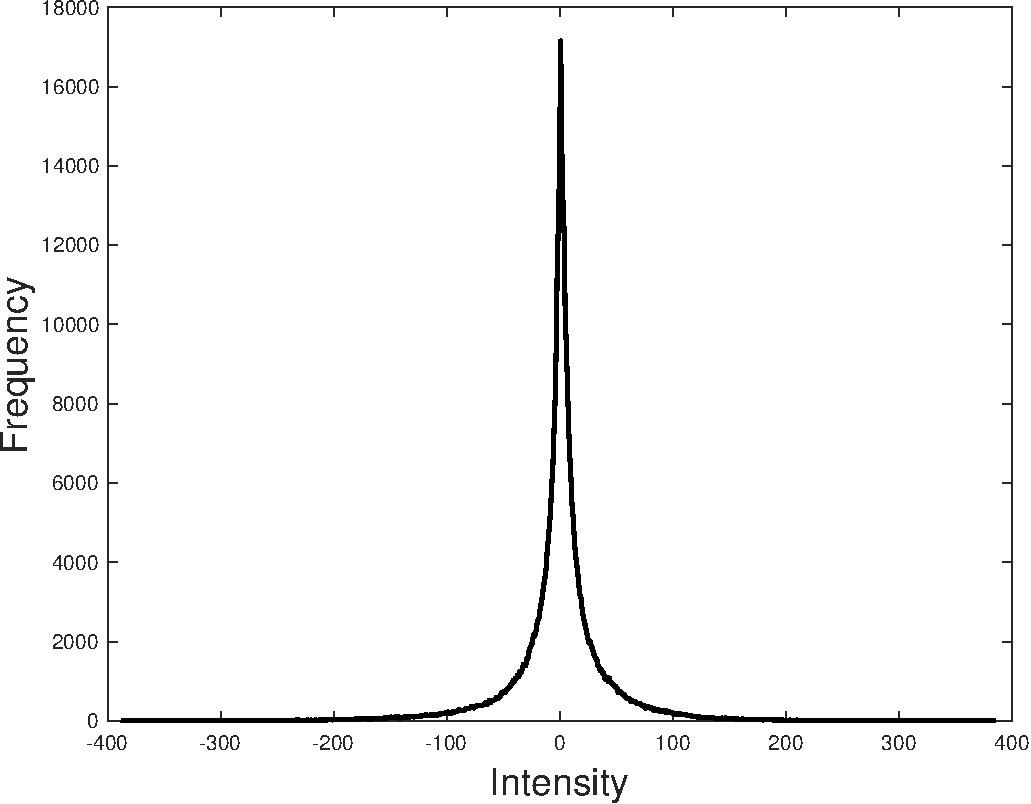
\includegraphics[width=\textwidth]{figures/statistical_image_models/spain_dy_histogram.pdf}
    \end{subfigure}
\caption{Top row:  image, and horizontal and vertical derivatives of the image.  Bottom row:  histogram of each image in top row.  Note that the histograms of the two bandpass filtered versions of the original image have the non-Gaussian distributions characteristic of natural images.} 
\label{fig:derivativeshist}
\end{figure}
\end{comment}

\begin{figure}[t]
\centerline{
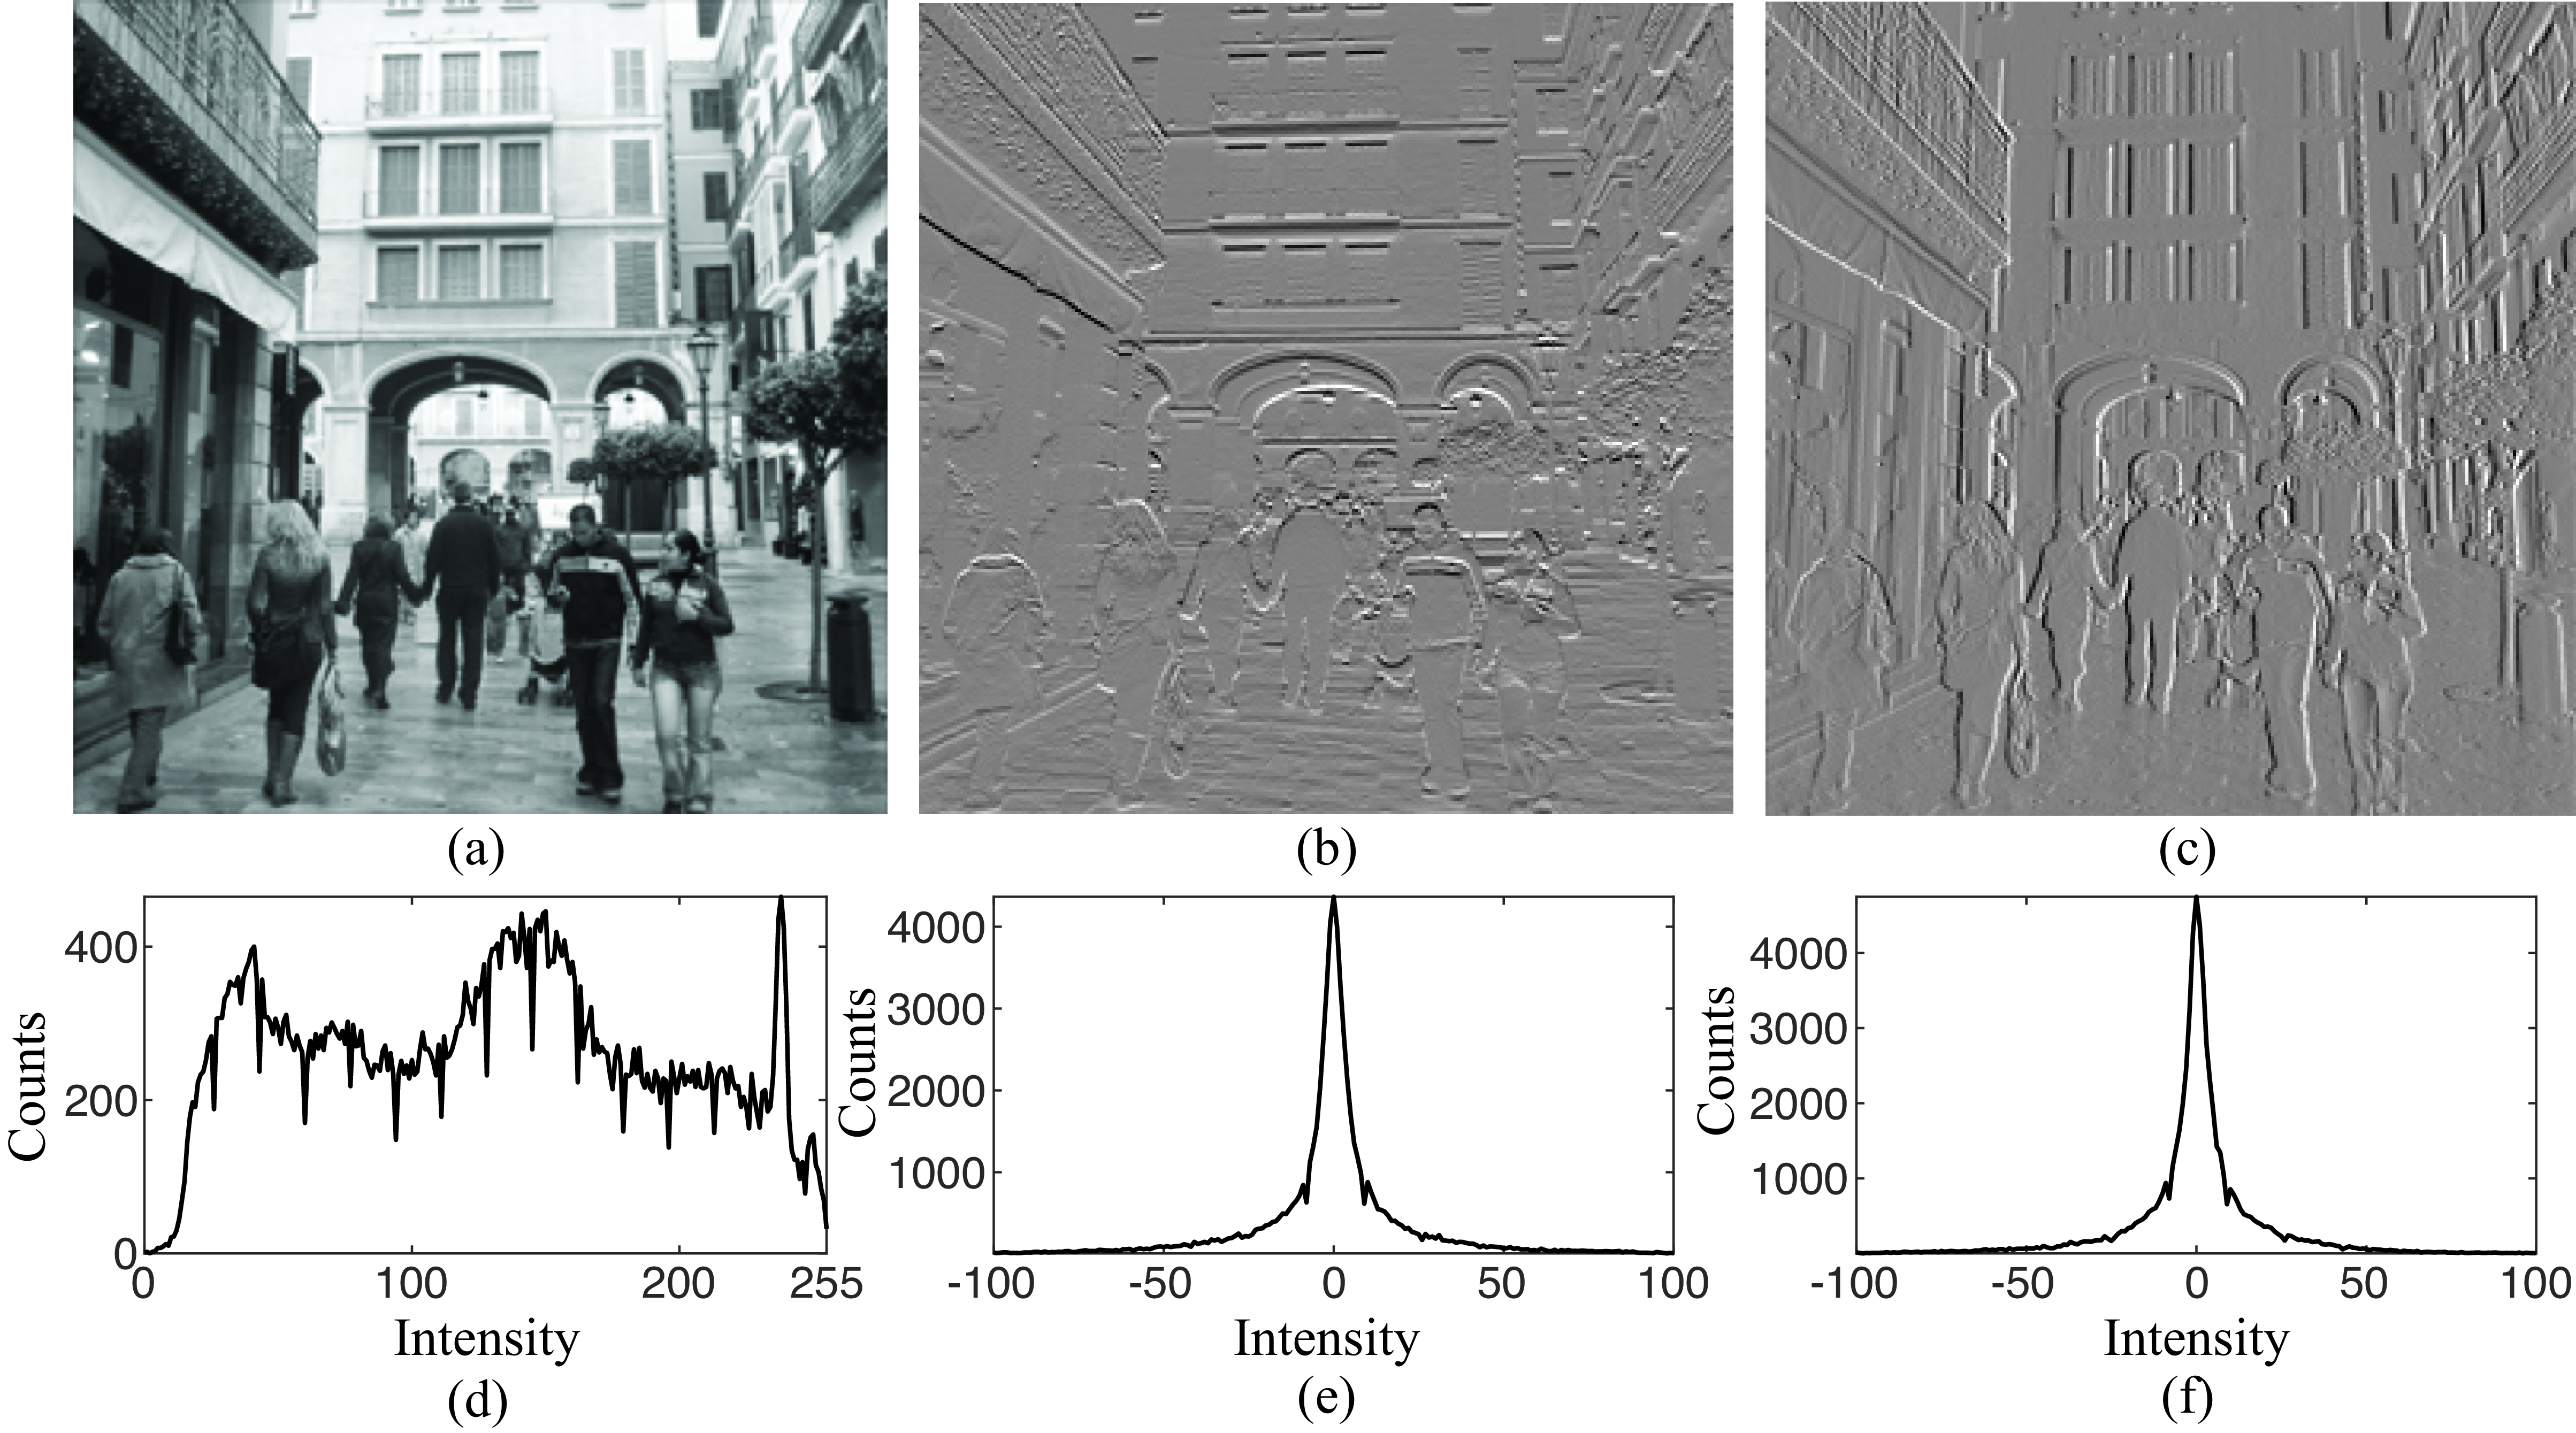
\includegraphics[width=1\linewidth]{figures/statistical_image_models/figure_histograms_derivatives_street.eps}
} 
\caption{(a) Input image.  (b) Horizontal and (c) vertical derivatives of the input image.  (d) Histogram of pixel intensities of the input image.  (e and f) Histograms of the two derivatives of the original image. Note that both histograms have non-Gaussian distributions, a characteristic of natural images.} 
\label{fig:derivativeshist}
\end{figure}



First, the histogram of an unfiltered image is already non-Gaussian. However, the image histogram does not have any interesting structure and different images have different histograms. Something very different happens to the outputs of the filters  $\left[-1,1\right]$ and $\left[-1,1\right]^\transpose$. The histograms of the filter outputs are very clean (note that they are computed over the same number of pixels), have a unique maximum around zero, and seem to be symmetric.

Note that this distribution of the filter outputs goes against the hypothesis of the Gaussian model. If the Gaussian image model were correct, then any filtered image would also be Gaussian, as a filtering is just a linear operation over the image.     \Fig{\ref{fig:derivativesdistributions}} makes this point, showing histograms of band-pass filtered images (an image containing Gaussian noise, and two natural images).  Note that the image subband histograms are significantly different than Gaussian.

\begin{figure}[t]
\centerline{
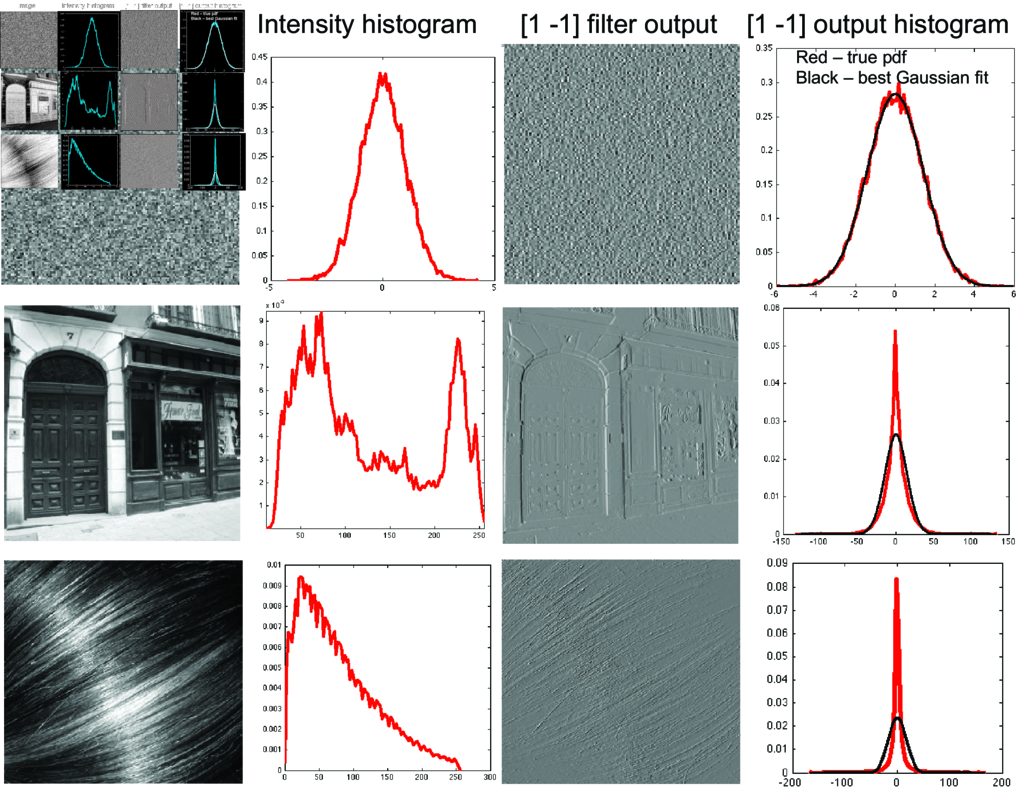
\includegraphics[width=1\linewidth]{figures/statistical_image_models/examplesderivativedistributions.eps}
} 
\caption{Comparison of histograms of images from different visual worlds, and band-pass filtered versions of those images. (top row) Gaussian noise.  Band-pass filtered Gaussian noise is still Gaussian distributed.  (middle and bottom rows) Two very different looking images, when band-pass filtered, have similar looking non-Gaussian, narrowly peaked histogram distributions. The black line shows the best Gaussian fit, a poor fit to the spiky histograms.} 
\label{fig:derivativesdistributions}
\end{figure}


The distribution of intensity values in the image filtered by a band-pass filter $h$, $\boldimg_h = \boldimg \circ \mathbf{h}$, can be parameterized by a simple function:
\begin{equation}
p(\img_h[n,m] = x) = \frac{\exp \left(- \left| x/s  \right|^r \right)}{2 (s/r) \Gamma(1/r)}
\label{eq:derdist}
\end{equation}

Where $\Gamma$ is the Gamma distribution. This function, \eqn{\ref{eq:derdist}}, known as the generalized Laplacian distribution, has two parameters: the exponent $r$, which alters the distribution's shape; and the scale parameter $s$, which influences its variance. This distribution fits the outputs of band-pass filters of natural images remarkably well. In natural images, typical values of $r$ lie within the range $\left[0.4, 0.8\right]$.

\marginnote{The standard Laplacian distribution has the form:
\begin{equation*}
p(x) = \frac{1}{2} \exp \left(- \left| x \right| \right)
\end{equation*}
}[-1in]

%\begin{comment}
\Fig{\ref{fig:generalizedgaussian}} shows the shape of the distribution when changing the parameter $r$. Setting $r=2$ gives the Gaussian distribution. With $r=1$ we obtain the standard Laplacian distribution.
When $r \to \infty$ the distribution converges to a uniform distribution in the range $\left[-s, s\right]$. And when $r \to 0$, the distribution converges to a delta function.
\begin{figure}[h]
\centerline{
\includegraphics[width=1\linewidth]{figures/statistical_image_models/shapes_generalized_laplacian.eps}
} 
\caption{Generalized Laplacian distribution with $s=1$ and (a) $r=0.1$, (b) $r=1$, (c) $r=2$, and (d) $r=10$. %Changing the exponent $r$ changes the shape of the distribution, generating some special case probability distributions (Gaussian, uniform, Laplacian).
} 
\label{fig:generalizedgaussian}
\end{figure}
%\end{comment}

%Note that for $r = 2$, this model becomes the gaussian model.


%Some properties of this distribution:
%\begin{eqnarray}
%mean = 0\\
%var = \\
%kurtosis = \\
%\end{eqnarray}

%Sometimes, vertical derivatives could be skewed due to illumination effects. Find one example.

%FIGURE: Compare the distribution obtained with different visual worlds (clouds, images, gaussian noise). Change the fit so that it uses the generalized gaussian.




% There are other prior distributions that also fit well the data.



Now that we have seen that image derivatives follow a special distribution for natural images, let's define a statistical image model that captures the distribution of image derivatives. We can use this prior model in synthesis and noise cleaning applications.

Let's consider a filter bank of $K$ filters with the convolution kernels: $h_k [n,m]$ with $k=0, ..., K-1$. The filter bank could be composed of several Gaussian derivatives with different orientations and orders, or Gabor filters, or steerable filters from the steerable pyramid, or any other collection of band-pass filters. If we assume that the output of each filter is independent from each other (clearly, this assumption is only an approximation) we can write the following prior model for natural images:
\begin{equation}
p(\boldimg) = \prod_{k=0}^{K-1} \prod_{n,m} p_k(\img_k [n,m])
% p(h_k(\mathbf{x}, n,m))
\label{eq:waveletmodel}
\end{equation}
This distribution is the product over all filters and all locations, of how likely is each filtered value according to the distribution of natural images as modeled by the distributions $p_k$, where $p_k$ is a distribution with the form from \eqn{\ref{eq:derdist}}. 


\marginnote{What is the most likely image under the model \eqn{\ref{eq:waveletmodel}}? It is a constant image.}

To see how this model works, let's look at a toy problem. 

\subsection{Toy Model of Image Inpainting}

%\begin{examples} {\bf step edge}

To build intuition about image structures that are likely under the wavelet marginal model, let's consider a simple 1D image of length $N=11$ that has a missing value in the middle:
\begin{equation}
\boldimg = \left[1,~ 1,~ 1,~ 1,~ 1,~ ?,~ 0,~ 0,~ 0,~ 0,~ 0\right]
\end{equation}
The middle value is missing because of image corruption or occlusion and we want to guess the most likely pixel intensity at that location. This task is called {\bf image inpainting}. In order to guess the value of the missing pixel we will use the image prior models we have presented in this chapter. 

We will denote the missing value with the variable $a$. Different values of $a$ will produce different types of steps. For instance, setting $a=1$ or $a=0$ will produce a sharp step edge. Setting $a=0.5$ will produce a smooth step signal. What is the value of $a$ that maximizes the probability of this 1D image under the wavelet marginal model? 

First, we need to specify the prior distribution. For this example we will use a model specified by a single filter ($K=1$) with the convolution kernel $[-1, 1]$, and we will use the distribution given by equations (\ref{eq:derdist}) and (\ref{eq:waveletmodel}). In this case, we can write the wavelet marginal model from \eqn{\ref{eq:waveletmodel}} in close form. Applying the filter $\left[-1, 1\right]$ to the 1D signal and using mirror boundary conditions, results in:
\begin{equation}
\boldimg_0 = \boldimg \circ \left[-1, 1\right] = \left[0,~0,~ 0,~0,~ 0,~ 1-a,~ a,~ 0,~ 0,~ 0,~ 0\right]
\end{equation}

Now, we can use \eqn{\ref{eq:waveletmodel}} to obtain the probability of $\boldimg$ as a function of $a$:
\begin{eqnarray}
p(\boldimg \given a) &=& \prod_{n=0}^{N-1} p(\img_0 [n]  \given a) = \\ %= \prod_{n} p(y [n]) \\
&=&\frac {\exp \left(- \left| (1-a)/s  \right|^r \right) \exp \left(- \left| a/s  \right|^r \right)}{(2s/r \Gamma(1/r))^N} =\\
&=&\frac{1}{(2s/r \Gamma(1/r))^N} \exp - \frac{\left| 1-a \right|^r+\left| a \right|^r} {s^r}  
\label{eq:best_a_eqn}
\end{eqnarray}
Note that the first factor only depends on $r$ and on the signal length $N$, and the second factor depends on $r$ and the missing value $a$. We are interested in finding the values of $a$ that maximize the $p(\boldimg \given a)$ for each value of $r$. Therefore, only the second factor is important for this analysis. \Fig{\ref{fig:surface_best_a}} plots the value of the second factor of \eqn{\ref{eq:best_a_eqn}} as we vary $a$ and $r$. The red line represent the places where the function reaches a local maximum as a function of $a$ for every value of $r$.

\begin{figure}[t]
\centerline{
\includegraphics[width=.6\linewidth]{figures/statistical_image_models/best_a_s1.eps}
} 
\caption{Best values of $a$, as a function of $r$, that maximize the probability of the 1D image $\left[1,1,1,1,1,a,0,0,0,0,0 \right]$ under the wavelet prior model. The optimal $a$ changes when crossing the $r=1$ value.} 
\label{fig:surface_best_a}
\end{figure}

For $r=2$ the best value of $a$ is $a=0.5$, and this solution is the best for any value of $r>1$. For $r=1$, any value $a \in \left[0,1\right]$ is equally good, and $p(\boldimg)$ decreases for values of $a$ outside that range. And for $r<1$, the best solution is for $a=0$ or $a=1$. Therefore, values of $r<1$ prefer sharp step edges. Note that $a=0$ and $a=1$ are both the same step edge translated by one pixel. 

\Fig{\ref{fig:best_a}} shows the final result using two different values of $r$. When using $r=2$, the result is a smooth signal (which is the same output we would had gotten if we had used the Gaussian image prior). The estimated value for $a$ is the average of the nearby values. For $r=0.5$, the result is a sharp step edge. The estimated value of $a$ can be equal to any of the two nearby values. In the plot shown in \fig{\ref{fig:best_a}}(right) corresponds to taking the value $a=1$. 

\begin{figure}[h]
\centerline{
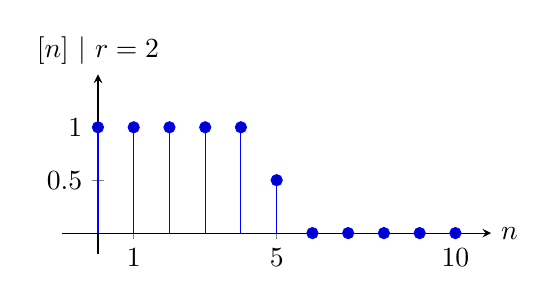
\begin{tikzpicture}
\begin{axis} [width=200pt,height=110pt,
	axis x line=middle, 
	axis y line=middle, 
	tick align=center,
	every axis x label/.style={at={(current axis.right of origin)},anchor=west},
	every axis y label/.style={at={(current axis.above origin)}, anchor=north east,above=0mm},
	xmin=-1, xmax=11,
	xtick={0, 1, 5, 10},
	xlabel=$n$,
	ymin=-0.2, ymax=1.5,
	ytick={0, 0.5, 1},
	ylabel={$\img [n]  ~|~  r=2$},
	color=black]
\addplot+[ycomb] plot coordinates {(0, 1) (1, 1) (2, 1) (3, 1) (4, 1) (5, 0.5) (6, 0) (7, 0) (8, 0) (9, 0) (10, 0)};
\end{axis} 
\end{tikzpicture}
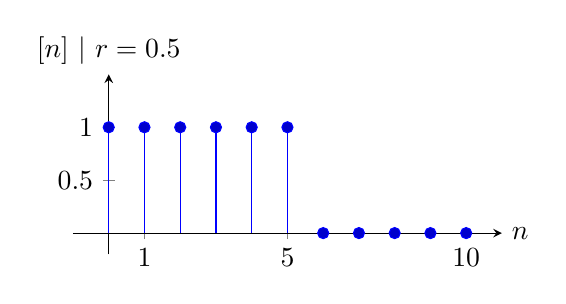
\begin{tikzpicture}
\begin{axis} [width=200pt,height=110pt,
	axis x line=middle, 
	axis y line=middle, 
	tick align=center,
	every axis x label/.style={at={(current axis.right of origin)},anchor=west},
	every axis y label/.style={at={(current axis.above origin)}, anchor=north east,above=0mm},
	xmin=-1, xmax=11,
	xtick={0, 1, 5, 10},
	xlabel=$n$,
	ymin=-0.2, ymax=1.5,
	ytick={0, 0.5, 1},
	ylabel={$\img [n]  ~|~ r=0.5$},
	color=black]
\addplot+[ycomb] plot coordinates {(0, 1) (1, 1) (2, 1) (3, 1) (4, 1) (5, 1) (6, 0) (7, 0) (8, 0) (9, 0) (10, 0)};
\end{axis} 
\end{tikzpicture}
}
\caption{Reconstructed signal using (left) $r=2$ and (right) $r=0.5$. The estimated values of $a$ are 0.5 and 1.} 
\label{fig:best_a}
\end{figure}



%%% HEEGER/BERGEN was here.

\subsection{Image Denoising (Bayesian Image Estimation)}

The highly kurtotic distribution of band-pass filter responses in images provides a regularity that is very useful for image denoising.  
If we assume zero-mean additive Gaussian noise of variance $\sigma^2$, and the observed subband coefficient value $\hat{x} = \hat\img_0 [n,m]$, where $\hat\img_0 [n,m]$ is the subband of the observed noisy input image, then the likelihood of any coefficient value, $x=\img_0 [n,m]$, is
\begin{equation}
p(\hat{x} \given x) \propto \exp{ \left( -\frac{(x - \hat{x})^2}{2 \sigma^2} \right) }, 
\end{equation}
where we are suppressing the normalization constants of \eqn{\ref{eq:derdist}} for simplicity.
The prior probability of any coefficient value is the Laplacian distribution (assuming $r=1$) of the subbands,
\begin{equation}
p(x) \propto \exp{ \left( -\frac{\left| x \right|}{s} \right) }.
\end{equation}
By Bayes rule, the posterior probability is the product of those two functions, 
\begin{equation}
P(x \given \hat{x}) \propto \exp{ \left( -\frac{\left| x \right|}{s} \right)} \exp{ \left( -\frac{(x - \hat{x})^2}{2 \sigma^2} \right) }
\label{eq:posterior_w_given_y}
\end{equation}

The plots of \fig{\ref{fig:waveletBayes}} show how this works.  The horizontal axis for each plot is the value at a pixel of an image subband coefficient.  The blue curve, showing the Laplacian prior probability for the subband values, is the same for all rows. The red line is the Gaussian likelihood and it is centered in the observed coefficient, and it is proportional to the probability that the true value had any other coefficient value. The green line shows the posterior, \eqn{\ref{eq:posterior_w_given_y}}, for several different coefficient observation values.  \Fig{\ref{fig:waveletBayes}}{a} shows the result when a zero subband coefficient is observed, resulting in the zero-mean Gaussian likelihood term (red), and the posterior (black) with a maximum at zero.  In \fig{\ref{fig:waveletBayes}}{b} an observation of 0.26 shifts the likelihood term, but the posterior still has a peak at zero.  And in \fig{\ref{fig:waveletBayes}}{c} an observed coefficient value of 1.22 yields a maximum posterior probability estimate of 0.9.


\begin{figure}
\centerline{
\includegraphics[width=.9\linewidth]{figures/statistical_image_models/wavelet_denoising.eps}
}
%\includegraphics[width=0.7\linewidth]
%{figures/statistical_image_models/x0wavelet.pdf}}
%\centerline{
%\includegraphics[width=0.7\linewidth]
%{figures/statistical_image_models/x1wavelet.pdf}}
%\centerline{
%\includegraphics[width=0.7\linewidth]
%{figures/statistical_image_models/x3wavelet.pdf}}
\caption{Showing the likelihood, prior, and posterior terms for the estimation of a subband coefficient from several noisy observations.  (a)  A zero subband coefficient is observed. (b)  An observation of 0.26 shifts the likelihood term, but the posterior still has a peak at zero. (c) an observed coefficient value of 1.22 yields a maximum posterior probability estimate of 0.9.
}
\label{fig:waveletBayes}
\end{figure}


\Fig{\ref{fig:bayeslut}} shows the resulting look-up table to modify the noisy observation to the MAP estimate for the denoised coefficient value.  Note that this implements a {\bf coring function} \cite{Simoncelli96}:  if a coefficient value is observed near zero, it is set to zero, based on the very high prior probability of zero coefficient values. 


\begin{figure}
\centerline{
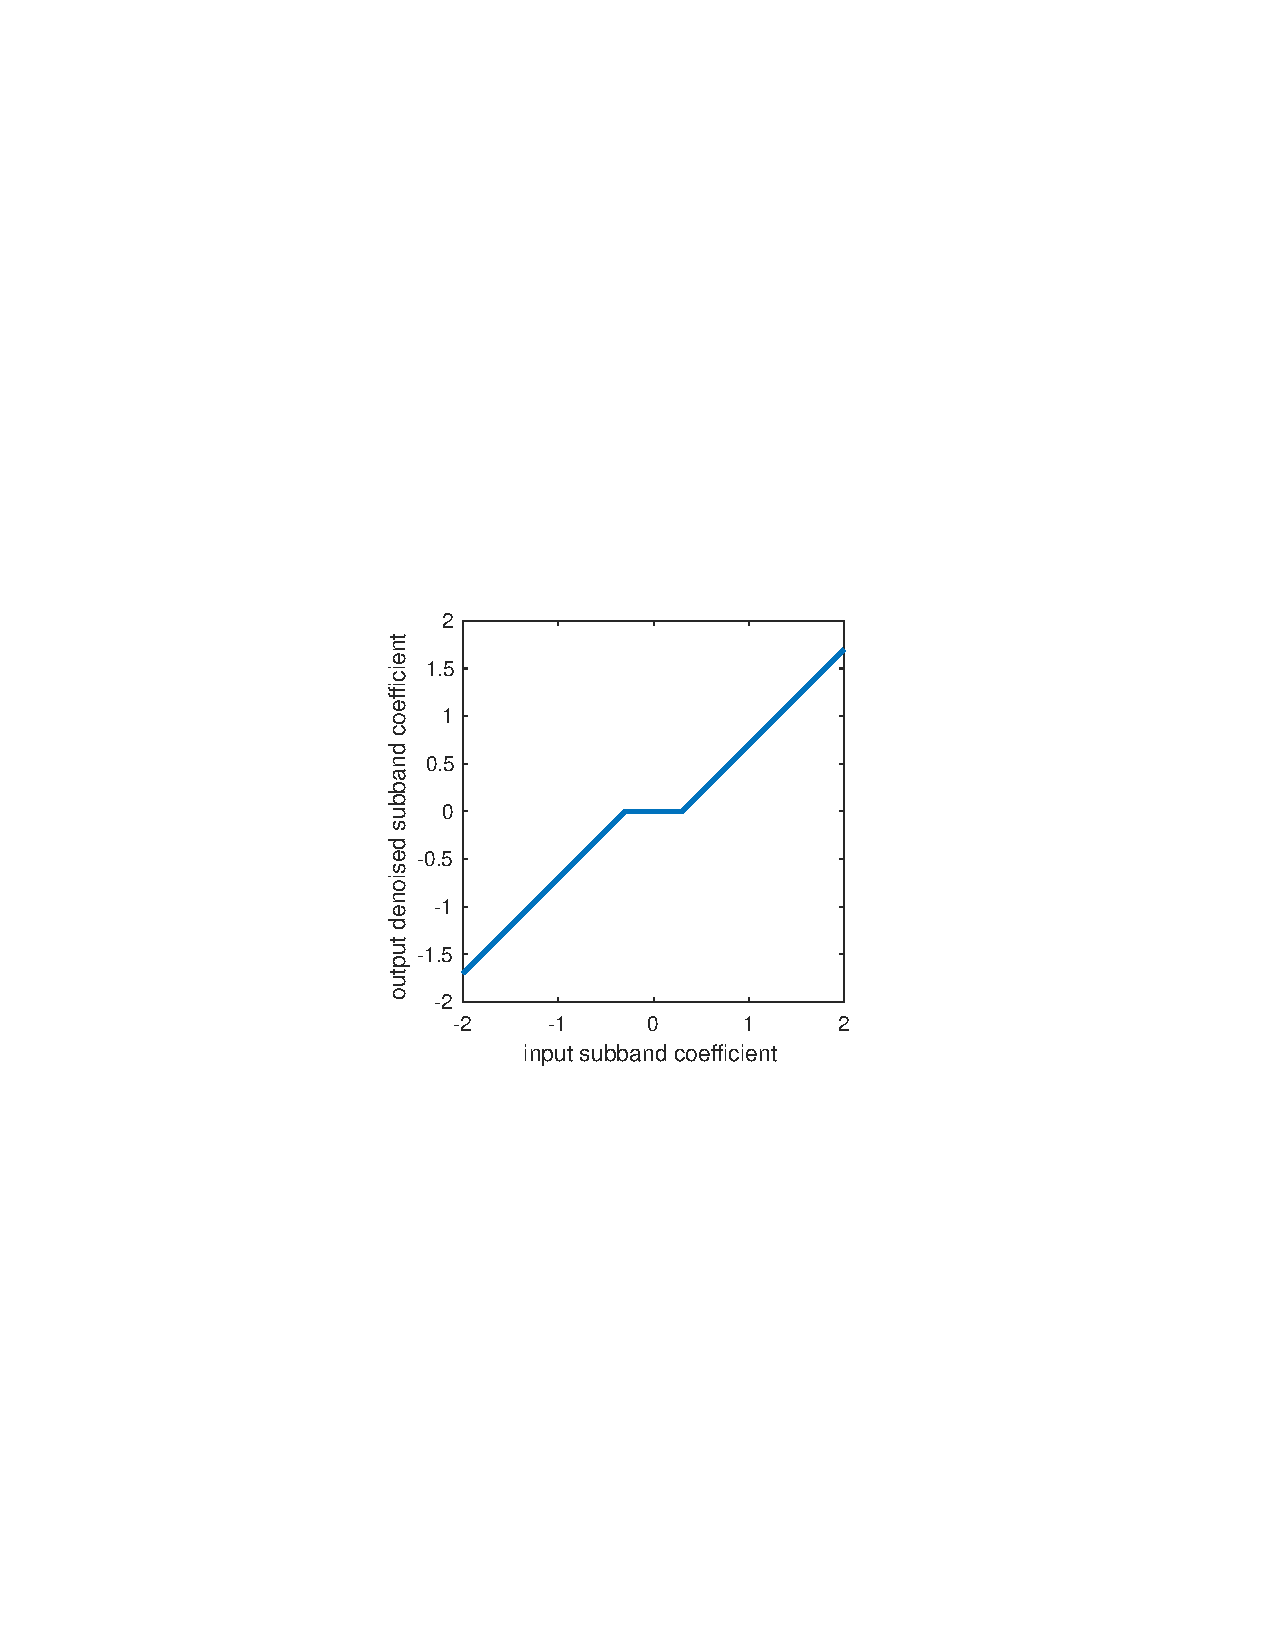
\includegraphics[width=0.4\linewidth]{figures/statistical_image_models/waveletlut.pdf}
}
\caption{Input/output coring curve for maximum posterior denoising for the example of \fig{\ref{fig:waveletBayes}}.
}
\label{fig:bayeslut}
\end{figure}

For a more detailed analysis and examples of denoising using the Laplacian image prior, we refer the reader to the work of Eero Simoncelli \cite{Simoncelli96}.

\section{Nonparametric Markov Random Field Image Models}

The Gaussian and kurtotic wavelet image priors both involve modeling the image as a sum of statistically independent basis functions, Fourier basis functions, in the case of the Gaussian model, or wavelets, in the case of  the wavelet image prior. 

A powerful class of image models is known as {\bf Markov random field} (MRF) models.  They have a precise mathematical form, which we will describe later, in \chap{\ref{chapter:probabilistic_graphical_models}}.  For now, we present the intuition for these models:  if the values of enough pixels surrounding a given pixel are specified, then the probability distribution of the given pixel is independent of the other pixels in the image.  To fit and sample from the MRF structure requires the mathematical tools of graphical models, to be introduced in \chap{\ref{chapter:probabilistic_graphical_models}}.

%, but here we present an algorithm, introduced by Efros and Leung \cite{Efros99} that exploits intuitions about the Markov structure of images to synthesize textures that are visually compelling.  



%\subsection{Denoising model (Non-local Means)}
%The image generation method of Efros and Leung has a natural denoising counterpart.  
As we will see in the following chapter,  Efros and Leung \cite{Efros99} introduced an algorithm for texture synthesis that exploits intuitions about the Markov structure of images to synthesize textures that are visually compelling.
The intuition of the Efros and Leung texture generation model is that if you condition on a large enough region of nearby pixels around a center pixel, that effectively determines the value of the central pixel. We will study this algorithm in more detail in the next chapter devoted to texture analysis and synthesis (\chap{\ref{chap:textures}}). We will focus here on a similar algorithm for the problem of image denoising.  

\subsection{Denoising Model (Nonlocal Means)}

Baudes, Coll, and Morel made use of that intuition to define the {\bf nonlocal means} denoising algorithm \cite{Baudes2005}. \index{Nonlocal means}
The nonlocal means denoised image is a weighted sum of all other pixels in the image, weighted by the similarity of the local neighborhoods of each pair of pixels.  More formally, 
\begin{equation}
    \img_{\mbox{NLM}}[n,m] = \sum_{k,l} w_{n,m}[k,l] \img [k,l]
\end{equation}
where
\begin{equation}
    w_{n,m}[k,l] = \frac{1}{Z_{n,m}} \exp{\frac{- \left| \img [N_{k,l}] - \img [N_{n,m}] \right| ^2}{h^2}},
    \label{fig:mask}
\end{equation}
where $N_{i, j}$ denotes an $h \times h$ region of pixels centered at $i, j$, and $Z_{n,m}$ is set so that the weights over the image sum to one, that is $\sum_{kl} w_{n,m}[k,l] = 1$.


%Left:  original image.  Middle: With additive Gaussian noise added, $\sigma=15$ for 0-255 image scale. Left: Non-local means noise removed result. 

% **********************
% august 29, 2021.  see numtour.m   to do:  look at the histograms (change the figs flag) for meanFlag = 0 % and nois level = 0.0111.  do these parameters make visual sense with all the plots??
% **********************



\Fig{\ref{fig:nlm1}} shows the weighting functions for two images. The parameter $h$ is typically set to $10 \sigma $, where $\sigma$ is the estimated image noise standard deviation. Within figures \ref{fig:nlm1}(a and b) at left is a grayscale image where the center position of interest to be denoised is marked with a white star.  The right side of the figures shows for some value of $h$ in \eqn{\ref{fig:mask}} the weighting function $w_{n,m}[k,l]$ indicating which pixels are averaged together to yield the nonlocal mean value placed at the starred location in the denoised image.  Note, for both figures \ref{fig:nlm1}(a and b) the sampling at image regions with similar local structure as the image position to be denoised.


\begin{figure}[t]
\centerline{
\sublabel{a}{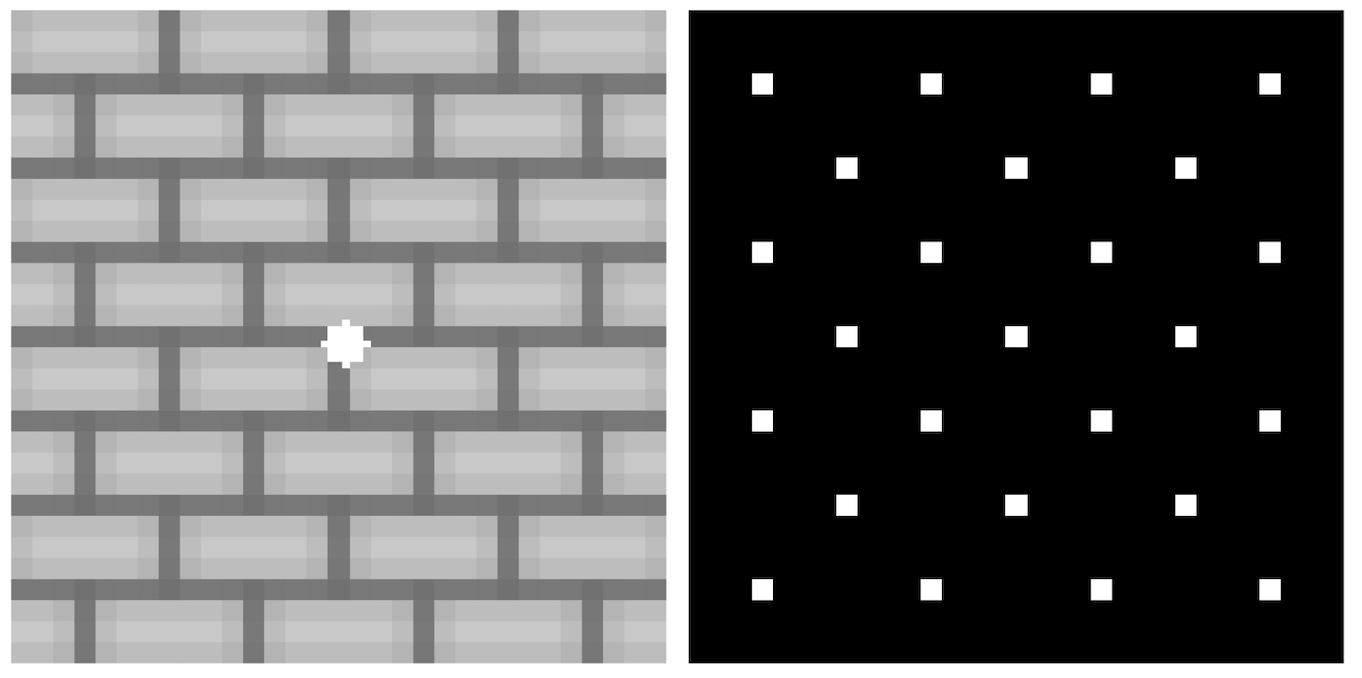
\includegraphics[width=0.48\linewidth]{figures/statistical_image_models/nlm1a.jpg}}
\sublabel{b}{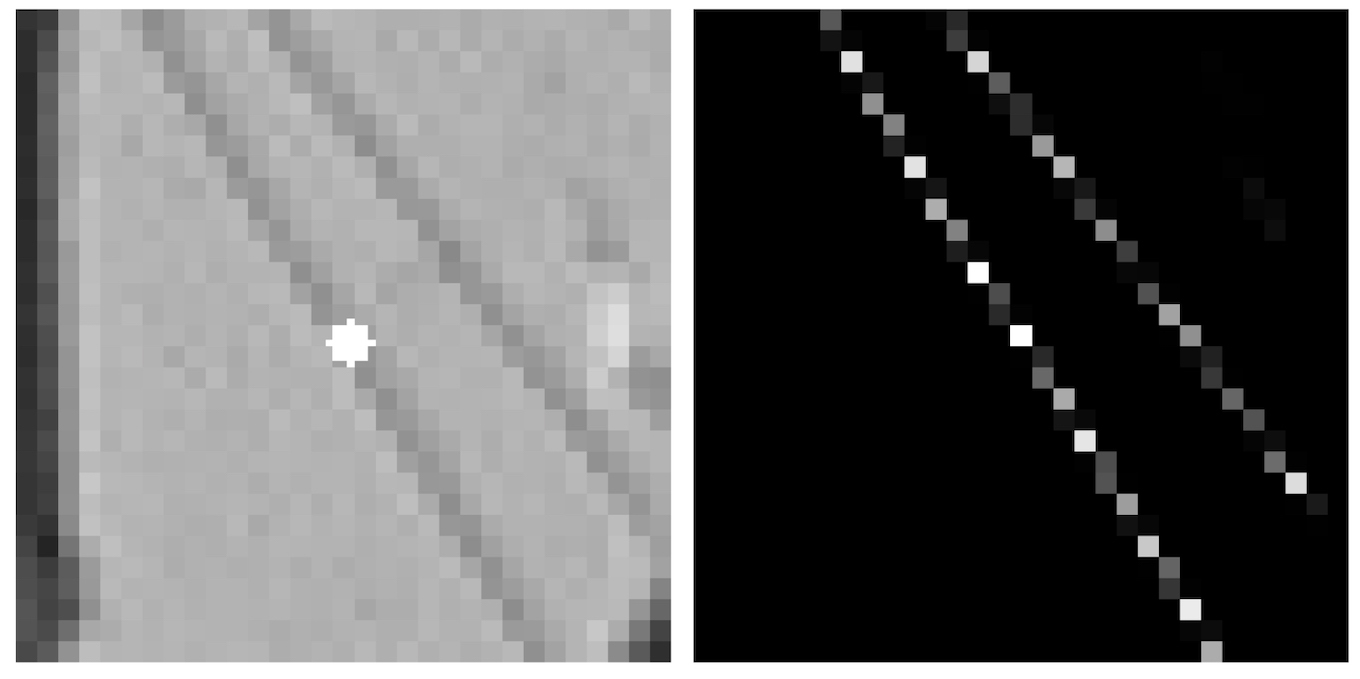
\includegraphics[width=0.48\linewidth]{figures/statistical_image_models/nlm1b.jpg}}
}
\caption{Regions of support for the nonlocal means denoising algorithm. 
{\em Source:} Image from \cite{Baudes2005}.}
\label{fig:nlm1}
\end{figure}

\Fig{\ref{fig:nlm2}} shows the result on a real image.  On the left is the original image. The middle image is with additive Gaussian noise added, that is, $\sigma=15$ for 0–255 image scale. On the right is the result, showing the image with nonlocal means noise removed.


\begin{figure}[t]
\centerline{
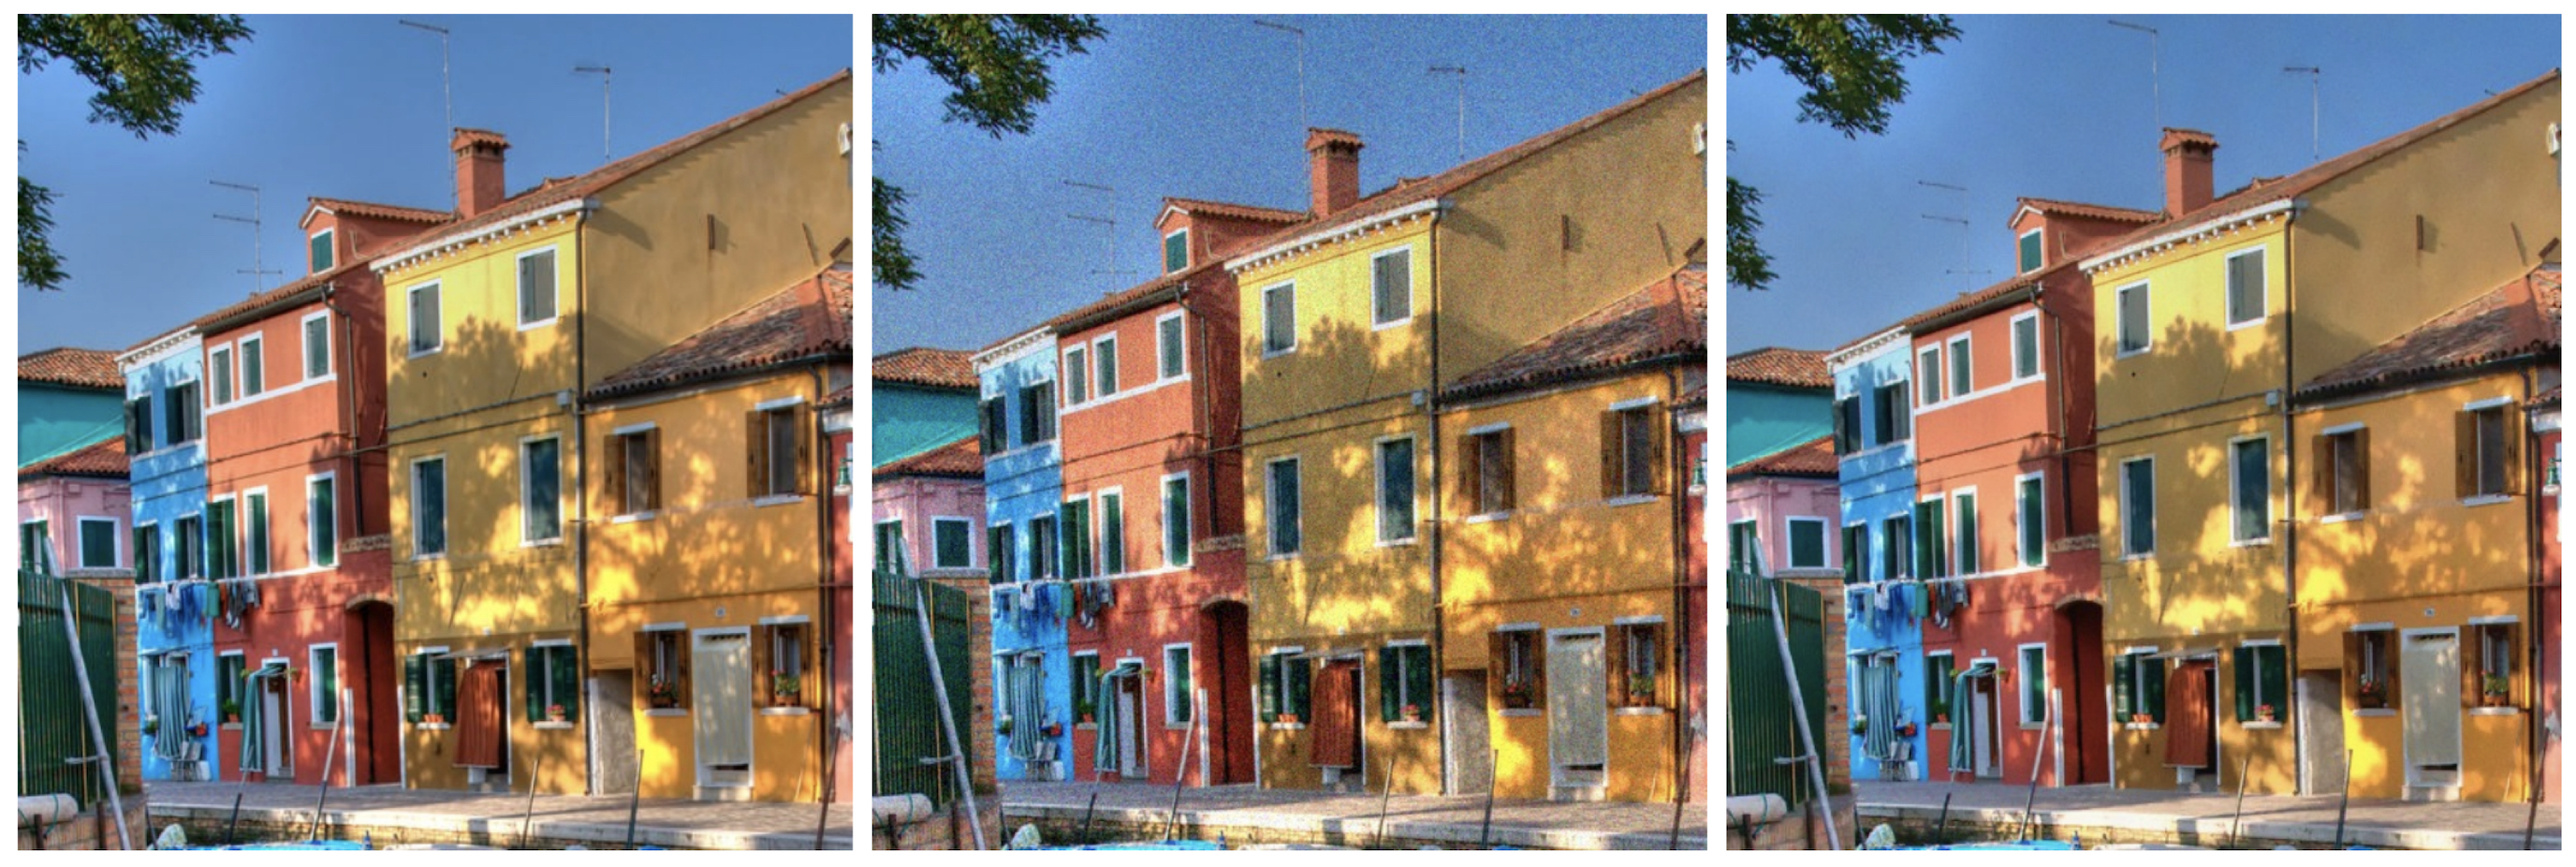
\includegraphics[width=1\linewidth]{figures/statistical_image_models/nlmresult.jpg}
}
\caption{Nonlocal means denoising algorithm results. (left) Original image without noise. (middle) Noisy image. (right) Denoised image. {\em Source:} Figure from \cite{Baudes2011}.
}
\label{fig:nlm2}
\end{figure}


% Observations: if $r = 2$, then this model becomes the gaussian model.


%\subsubsection{Examples}
%
%
%Example of a 1D step edge and sharpening. See the effect of p in what is the best solution.
%

% First, what is the most likely image under the model eq.~\ref{eq:waveletmodel}. It is a constant image. 

%\begin{examples} {\bf step edge}

% To build an intuition on what types of image structures are more likely under the wavelet marginal model, let's consider a simple 1D image:
% \begin{equation}
% \img = \left[1,~ 1,~ 1,~ a,~ 0,~ 0,~ 0\right]
% \end{equation}
%Different values of $a$ will produce different types of steps. For instance, setting $a=1$ or $a=0$ will produce a sharp step edge. Setting $a=0.5$ will produce a smooth step signal. What is the value of $a$ that maximizes the probability of this 1D image under the wavelet marginal model? 

%First we need to specify the prior distribution. For this example we will use a model specified by a single filter with the form $[-1, 1]$, and we will use the distribution given by eq.~\ref{eq:derdist}. In this case, we can write the wavelet marginal model in close form. Applying the filter $\left[-1, 1\right]$ to the 1D signal and using mirror boundary conditions, results in:
%\begin{equation}
%h(\img) = \left[0,~0,~ 0,~ 1-a,~ a,~ 0,~ 0\right]
%\end{equation}

%Now, we can use Eq.~\ref{eq:waveletmodel} and obtain the probability of $\img$ as a function of $a$:
%\begin{eqnarray}
%p(\img) = \prod_{x} p(h(\img, x)) = \\
%\frac {\exp \left(- \left| (1-a)/s  \right|^r \right) \exp \left(- \left| a/s  %\right|^r \right)}{(2s/r \Gamma(1/r))^7} = \\
%\frac{1}{(2s/r \Gamma(1/r))^7} \exp - \frac{\left| 1-a \right|^r+\left| a %\right|^r} {s^r}  
%\end{eqnarray}
%the first factor only depends on $r$. The second factor depends on $a$ and $r$. We are interested in seeing the values of $a$ that maximize $p(\img)$ for each value of $r$. Therefore, only the second factor is important for this analysis. The next figure plots the value of the second factor as we vary $a$ and $r$. The red line represent the places where the function reaches a maximum as a function of $a$ for each value of $r$.

%\begin{figure}[htpb]
%\centerline{
%\includegraphics[width=.6\linewidth]{figures/statistical_image_models/best_a_s1.eps}
%} 
%\caption{Best values of $a$ that maximize the probability of the 1D image %$\left[1,~ 1,~ 1,~ a,~ 0,~ 0,~ 0\right]$ under the wavelet prior model.} 
%\label{fig:best_a}
%\end{figure}

%For $r=2$ the best value of $a$ is $a=0.5$, and this solution is the best for any value of $r>1$. For $r=1$, any value $a \in \left[0,1\right]$ is equally good, and $p(\img)$ decreases for values of $a$ outside that range. And for $r<1$, the best solution is for $a=0$ or $a=1$. Therefore, values of $r<1$ prefer sharp step edges. Note that $a=0$ and $a=1$ are both the same step edge translated by one pixel. 

%\end{examples} 
%
%\begin{examples}
%What happens if the signal has the form: $\img = \left[0,~ 1,~ 2,~ a,~ 4,~ 5,~ 6\right]$
%\end{examples} 
%
%\begin{examples}
%What happens if the signal has the form: $\img = \left[0,~ 0,~ 0,~ a,~ 0,~ 0,~ 0\right]$. (solution: $a=0$ for all $r$).
%\end{examples} 
%
%\begin{examples}
%What happens if we define other filters than $\left[-1, 1\right]$. For instance $\left[-1,~ 2,~ -1\right]$.
%\end{examples} 
%
%\example{Superresolution}
%
%\begin{equation}
%{\bf a} = [a_0,~a_1,~ a_2,~ a_3,~ a_4,~ a_5,~ a_6,~a_7]
%\end{equation}
%
%but we observe the signal:
%\begin{equation}
%{\bf b} = [b_0,~ b_1,~ b_2,~ b_3]
%\end{equation}
%obtained by filtering $\bf a$ with a filter $[1,~1]$ and then downsampling by a factor of 2. The process of going from $\bf a$ to $\bf b$ is linear.
%\begin{eqnarray*}
%b_0 = a_0+a_1\\
%b_1 = a_2+a_3\\
%b_2 = a_4+a_5\\
%b_3 = a_6+a_7\\
%\end{eqnarray*}
%
%Our goal is to recover the signal $\bf a$.
%
%\begin{equation}
%\bf a ^* = argmax_{\bf a} P(\bf a ~|~ \bf b)  = \frac{P(\bf b ~|~ \bf a) P(\bf a)}{P(\bf b)}
%\end{equation}
%
%If we consider only the feasible solutions, then the only term that matters to select the solution is the prior $P(\bf a)$.
%
%\begin{equation}
%h({\bf a}) = [0,~a_1-a_0,~ a_2-a_1,~ a_3-a_2,~ a_4-a_3,~ a_5-a_4,~ a_6-a_5,~ a_7-a_6]
%\end{equation}
%
%\begin{equation}
%h({\bf a}) = [0,   ~b_0-2 a_0, ~
%                    a_2-a_1,~ b_1-2 a_2,~ 
%                    a_4-a_3,~ b_2- 2 a_4,~ 
%                    a_6-a_5,~ b_3- 2 a_6]
%\end{equation}
%
%\begin{eqnarray}
%\log p({\bf a}) = \sum_{x} \log p(h(\bf a, x)) = \\
%- \left | (b_0-2 a_0)/s  \right|^r
%- \left | (a_2-a_1)/s  \right|^r - \left | (b_1-2 a_2)/s  \right|^r
%- \left | (a_4-a_3)/s  \right|^r - \left | (b_2-2 a_4)/s  \right|^r
%- \left | (a_6-a_5)/s  \right|^r - \left | (b_3-2 a_6)/s  \right|^r
%\end{eqnarray}

%\begin{examples}{\bf Image impainting}
%
%2D image with a missing block in the center.
%
%It is like having boundary conditions.
%
%$I = I_b \cup I_c$
%
%$p(I_c ~|~ I_b)$
%\end{examples}
%
%\begin{examples}{\bf Most natural image}
%Find the image from a database that maximizes the prior... What is the most natural image? Figure: show sorted images according to the prior.
%\end{examples}
%
%
%\begin{examples}{\bf Superresolution}
%One example for which we can not derive things analytically. Use iterative weighted least square to do inference. Check effect on the exponent p on the solution.
%\end{examples}
%
%


%\section{Sparsity}

%Talk about Field and Olshausen, and establish parallelism with CNN.


%\subsubsection{Cooring: Denoising with the wavelet model}

%Deduce Wavelet thresholding using the bayesian model.

%In the case of $\left[-1, 1\right]$ derivatives we can transform the image, then apply the prior to the derivatives, and then reverse the transformation. 

%
%\subsubsection{Retinex}
%
%Try a sequence of models:
%
%1) gaussian
%
%2) laplacian
%
%3) laplacian + gaussian on second order derivatives
%
%
%
%is one step beyond denoting...
%
%Craik-O'Brien-Cornsweet effect
%
%
%\begin{figure}[htpb]
%\centerline{
%\includegraphics[width=1\linewidth]{figures/statistical_image_models/Cornsweeteffect.eps}
%} 
%\caption{Cornsweet effect.} 
%\label{fig:Cornsweeteffect}
%\end{figure}
%




%\subsection{Gaussian scale mixtures}


%\section{Patch based models}
%
%How do non-parametric image models fit in this?







%\section{Generative models in vision}
%
%As a more challenging task: a really complete model. Can it be done? I think there is a CNN by Renato trying to build also priors for images. Describe it here.
%
%Explaining away, sufficient statistics, nuisance parameters, ...

%
%
%\section{Applications of statistical image models}
%
%
%\subsection{Camera motion removal}
%
%\subsection{Separating image into intrinsic images}
%
%\subsection{Color demosaicing}
%
%
\section{Concluding Remarks}

The models presented in this chapter do not try to understand the content of the pictures, but utilize low-level regularities of images in order to build a statistical model.  Modeling these statistical regularities enable many tasks, including both image synthesis and image denoising.

We have see some simple models that try to constrain the space of natural images. These models, despite their simplicity, are useful in several applications. However, they fail in providing a strong image model that can be used to sample new images. As illustrated in \fig{\ref{fig:spaces_real_images_final}} the sequence of models we have studied in this chapter, only help in reducing a bit the space of possible images.


\begin{figure}
\centerline{
\includegraphics[width=1\linewidth]{figures/statistical_image_models/spaces_real_images_and_models_final.eps}
} 
\caption{The space of natural images is just very small part of the space of all possible images. In the case of color images with $32\times32$ pixels, most of the space is filled with images that look like noise.} 
\label{fig:spaces_real_images_final}
\end{figure}

We will see stronger generative image models in \chap{\ref{chapter:generative_models}}.

\begin{comment}
Figure~\ref{fig:synthesis} shows a random draw from the kurtotic wavelet statistical model of images \cite{Simoncelli2005}.  The long tails of the Laplacian subband distributions results in a small number of high-amplitude wavelet basis functions.  For the subband representation used here, the basis functions are x-y separable, giving the large amplitude, large-scale wavelets visible in the image.


\begin{figure}[htpb]
\centerline{
{\includegraphics[width=0.3\linewidth]{figures/statistical_image_models/waveletEero.pdf}}}
\caption{Random draw from wavelet model  \cite{Simoncelli2005}, for an x-y separable model composed of wavelets of many spatial scales.  Figure permission.
}
\label{fig:synthesis}
\end{figure}

\end{comment}